\documentclass[11pt,a4paper]{article}

% ─── Packages ────────────────────────────────────────────────────────────────
\usepackage[utf8]{inputenc}
\usepackage[T1]{fontenc}
\usepackage{lmodern}
\usepackage{geometry}
\usepackage{amsmath,amssymb,amsthm}
\usepackage{hyperref}
\usepackage{listings}
\usepackage{xcolor}
\usepackage{booktabs}
\usepackage{graphicx}
\usepackage{fancyhdr}
\usepackage{tikz}
\usetikzlibrary{arrows.meta,positioning,fit,backgrounds,calc,shapes.geometric,shapes.symbols,decorations.pathmorphing,decorations.pathreplacing}
\usepackage{float}
\usepackage{caption}
\usepackage{enumitem}

% ─── Geometry ────────────────────────────────────────────────────────────────
\geometry{margin=2.5cm}

% ─── Colors (hh-* harbor palette, identical to the Anchor paper) ──────────────
\definecolor{codebg}{RGB}{248,248,248}
\definecolor{codeframe}{RGB}{200,200,200}
\definecolor{darkgreen}{RGB}{0,100,0}
\definecolor{darkblue}{RGB}{0,50,100}
\definecolor{accent}{RGB}{0,128,128}
\definecolor{hhsand}{HTML}{E9DCC4}
\definecolor{hhsanddeep}{HTML}{D4C5A9}
\definecolor{hhebony}{HTML}{1E1B18}
\definecolor{hhink}{HTML}{2C2A26}
\definecolor{hhcinnabar}{HTML}{CC3D2E}
\definecolor{hhbrass}{HTML}{B08D57}
\definecolor{hhpatina}{HTML}{5C7A6A}
\definecolor{hhpaper}{HTML}{FBF7EE}

% ─── Honest-label key (ADR-0045 discipline; one key in every paper header) ────
\newcommand{\BUILT}{{\textcolor{hhpatina}{\textbf{\textsf{BUILT}}}}}
\newcommand{\BUILTWEAK}{{\textcolor{hhbrass}{\textbf{\textsf{BUILT-WEAK}}}}}
\newcommand{\DESIGNED}{{\textcolor{darkblue}{\textbf{\textsf{DESIGNED}}}}}
\newcommand{\VISION}{{\textcolor{hhcinnabar}{\textbf{\textsf{VISION}}}}}

% Verbatim-safe inline code for use INSIDE macro arguments (callouts, captions,
% TikZ nodes) where \verb is illegal. Detokenizes so special chars survive.
\newcommand{\code}[1]{{\ttfamily\detokenize{#1}}}

% Verification-status markers (kept for the appendix status table).
\newcommand{\Closed}{{\textcolor{hhpatina}{\textbf{\textsf{closed}}}}}
\newcommand{\Partial}{{\textcolor{hhbrass}{\textbf{\textsf{partial}}}}}
\newcommand{\Open}{{\textcolor{hhcinnabar}{\textbf{\textsf{open}}}}}

% Pull-quote sidebar: large quote, left-edge accent stripe.
\newcommand{\pullquote}[1]{%
  \par\vspace{6pt}%
  \noindent\begin{tikzpicture}
    \node[draw=none,fill=hhsand!40,line width=0pt,
          inner sep=10pt,text width=\dimexpr\textwidth-30pt\relax,
          align=left] (q) {%
      \sffamily\itshape\large #1%
    };
    \draw[hhcinnabar,line width=2.5pt] (q.north west) -- (q.south west);
  \end{tikzpicture}\par\vspace{6pt}%
}

% ─── Teaching callouts (new shared idiom, per Harbor Volume pedagogic spec) ───
% \keyidea{}: the load-bearing takeaway of a section, patina (sea-green) framed.
\newcommand{\keyidea}[1]{%
  \par\vspace{6pt}%
  \noindent\begin{tikzpicture}
    \node[draw=hhpatina,thick,fill=hhpatina!8,rounded corners=3pt,
          inner sep=9pt,text width=\dimexpr\textwidth-26pt\relax,align=left] (k) {%
      {\sffamily\bfseries\color{hhpatina} Key idea.}\enspace #1%
    };
  \end{tikzpicture}\par\vspace{6pt}%
}
% \pitfall{}: the way the idea is misread or mis-sold, cinnabar (red) framed.
\newcommand{\pitfall}[1]{%
  \par\vspace{6pt}%
  \noindent\begin{tikzpicture}
    \node[draw=hhcinnabar,thick,fill=hhcinnabar!7,rounded corners=3pt,
          inner sep=9pt,text width=\dimexpr\textwidth-26pt\relax,align=left] (p) {%
      {\sffamily\bfseries\color{hhcinnabar} Pitfall.}\enspace #1%
    };
  \end{tikzpicture}\par\vspace{6pt}%
}
% \exercises{}: end-of-section exercise block, sand-framed.
\newenvironment{exercises}{%
  \par\vspace{8pt}\noindent
  \begin{tikzpicture}
  \node[draw=hhbrass,thick,fill=hhsand!25,rounded corners=3pt,
        inner sep=10pt,text width=\dimexpr\textwidth-26pt\relax,align=left]
        \bgroup\begin{minipage}{\dimexpr\textwidth-46pt\relax}
  {\sffamily\bfseries\color{hhink}\large Exercises}\par\vspace{3pt}
  \small
}{%
  \end{minipage}\egroup;
  \end{tikzpicture}\par\vspace{8pt}
}

% ─── Listings Setup ──────────────────────────────────────────────────────────
\lstdefinestyle{pdcode}{
  language=C,
  backgroundcolor=\color{codebg},
  frame=single,
  rulecolor=\color{codeframe},
  basicstyle=\ttfamily\small,
  keywordstyle=\color{darkblue}\bfseries,
  commentstyle=\color{darkgreen}\itshape,
  stringstyle=\color{accent},
  numbers=left,
  numberstyle=\tiny\color{gray},
  numbersep=8pt,
  breaklines=true,
  showstringspaces=false,
  tabsize=2,
  xleftmargin=15pt,
  xrightmargin=5pt,
  framexleftmargin=15pt,
  captionpos=b
}
\lstset{style=pdcode}

% ─── Theorem Environments ────────────────────────────────────────────────────
\theoremstyle{definition}
\newtheorem{definition}{Definition}[section]
\newtheorem{theorem}{Theorem}[section]
\newtheorem{lemma}{Lemma}[section]
\newtheorem{property}{Property}[section]
\newtheorem{conjecture}{Conjecture}[section]

% ─── Header/Footer ───────────────────────────────────────────────────────────
\pagestyle{fancy}
\fancyhf{}
\fancyhead[L]{\small\textit{From Spawn to Person}}
\fancyhead[R]{\small\thepage}
\fancyfoot[C]{\small Port Daddy --- Harbor Volume, Paper 3 of 4 \quad\textbar\quad
  Honest labels: \BUILT~\textbar~\BUILTWEAK~\textbar~\DESIGNED~\textbar~\VISION}
\renewcommand{\headrulewidth}{0.4pt}
\renewcommand{\footrulewidth}{0pt}

% ─── Title ───────────────────────────────────────────────────────────────────
\title{
  \vspace{-1cm}
  {\Large\textsc{Technical White Paper --- Harbor Volume, Paper 3}}\\[0.5cm]
  \rule{\textwidth}{0.5pt}\\[0.3cm]
  {\LARGE\textbf{From Spawn to Person:}}\\[0.2cm]
  {\Large Identity, Continuity, and the Substrate\\of Agentic Reputation}\\[0.3cm]
  \rule{\textwidth}{0.5pt}
}
\author{
  \textbf{Erich Owens}\\[0.2cm]
  Curiositech LLC\\[0.2cm]
  \texttt{engineering@portdaddy.dev}
}
\date{June 2026\\Version 1.0 (Harbor Volume, L3 bridge)}

% ─── Document ────────────────────────────────────────────────────────────────
\begin{document}

\maketitle
\thispagestyle{empty}

\vspace{0.6cm}

\begin{abstract}\noindent
A coding-agent swarm produces work, but until that work can be attributed to
something that survives the process that did it, none of it can be priced. This
paper is the bridge of the Harbor Volume: it carries the through-line
\emph{memory $\to$ checkpoint $\to$ continuity $\to$ a person, not a spawn $\to$
witnessed outcomes $\to$ reputation $\to$ a tradeable asset} from the legible
single-operator tool (Papers~1--2) to the cross-operator market (Paper~4). We
make a single distinction load-bearing: a \textbf{role} is a bundle of
$\{\text{obligation}, \text{capability}, \text{authority}\}$ --- an org-chart
entry any spawn can fill --- while a \textbf{person} is a role instance
\emph{plus continuity}: durable memory, a restorable checkpoint, and a witnessed
history of outcomes keyed on an identity that cannot be freely re-picked. From
this we draw the volume's central economic claim, stated identically across the
papers: \emph{the reputation estimator is cheap; the substrate it scores over ---
witnessed outcomes on a non-forgeable identity --- is the gate.} We ground the
philosophy (Locke's memory criterion, Parfit's psychological continuity), name
the three continuity organs against shipped code with honest labels, and design
\textbf{ADR-0049}: a multi-dimensional reputation (accuracy / aesthetics /
efficiency, each a different axis with a different judge) scored by
\emph{neutral, conflict-free, influence-free} evaluators --- the harbor's
``universities and rating agencies'' --- hired through Port Daddy's own bonded
protocols. We argue at length why reputation is \emph{not} a bandit problem
(non-stationarity, multi-dimensionality, strategic adversaries, and the grading
oracle's own incentive-compatibility), and we treat the grading-oracle hole in
the core economic theorem head-on. We are disciplined about the keystone: this
paper depends on \textbf{ADR-0040 (identity-local)} and hands Paper~4 the unbuilt
\textbf{ADR-0040b (cross-operator attestation)} as a named dependency rather than
assuming it.
\end{abstract}

\vspace{0.5cm}
\noindent\textbf{Keywords:} agent identity, personal identity, psychological
continuity, reputation systems, mechanism design, Bradley--Terry, TrueSkill,
EigenTrust, LLM-as-judge, Sybil resistance, multi-armed bandits, incentive
compatibility, witnessed outcomes

\vspace{0.4cm}
\noindent\textit{Reading time: approximately 40 minutes end-to-end; the
Reader's Map below offers shorter routes. The companion papers \emph{The Legible
Swarm} (Paper~1, L2) and \emph{The Anchor Protocol} (Paper~2, L0--L1) supply the
legibility surfaces and the cryptographic identity ceremony this paper builds on;
\emph{The Harbor Economy} (Paper~4, L3) consumes this paper's reputation
substrate as the third side of its market. Any of the four can be opened first;
this one is the hinge.}

\vspace{0.3cm}
\noindent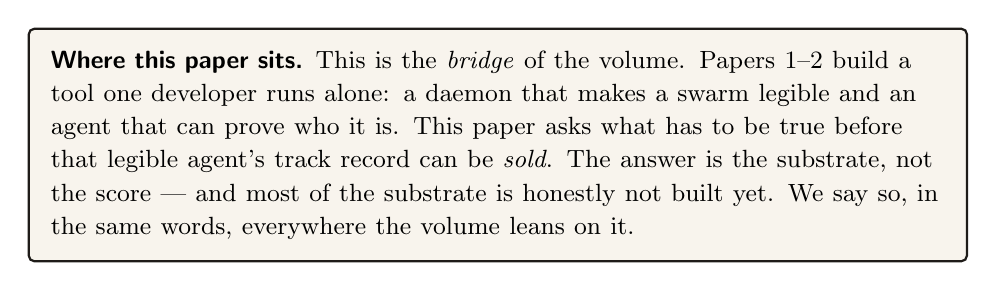
\begin{tikzpicture}
\node[draw=hhebony,thick,fill=hhsand!30,rounded corners=2pt,
      inner sep=8pt,text width=\dimexpr\textwidth-22pt\relax,
      align=left] (cbox) {%
  \small\textbf{\sffamily Where this paper sits.}\enspace This is the
  \emph{bridge} of the volume. Papers~1--2 build a tool one developer runs alone:
  a daemon that makes a swarm legible and an agent that can prove who it is. This
  paper asks what has to be true before that legible agent's track record can be
  \emph{sold}. The answer is the substrate, not the score --- and most of the
  substrate is honestly not built yet. We say so, in the same words, everywhere
  the volume leans on it.
};
\end{tikzpicture}

\tableofcontents
\newpage

% ═════════════════════════════════════════════════════════════════════════════
\section*{Reader's Map}\label{sec:readers-map}
\addcontentsline{toc}{section}{Reader's Map}
% ═════════════════════════════════════════════════════════════════════════════

\noindent The paper is one argument, but four kinds of reader want four different
routes through it. Each route names the load-bearing section and the artifact it
turns on.

\begin{table}[H]
\centering
\small
\renewcommand{\arraystretch}{1.35}
\begin{tabular}{@{}p{3.2cm} p{8.0cm} p{3.5cm}@{}}
\toprule
\textbf{If you are\ldots} & \textbf{Read} & \textbf{Turns on} \\
\midrule
A developer who runs one fleet &
\S\ref{sec:intro} (the spawn problem), \S\ref{sec:role-person} (role vs.\ person),
\S\ref{sec:organs} (what is built today). Skip the proofs. &
The honest-state table (Fig.~\ref{fig:honest-state}) \\
A philosopher / cognitive scientist &
\S\ref{sec:continuity} (Locke, Parfit, and why the \emph{ledger} not the
\emph{memory} is the identity organ), \S\ref{sec:organs}. &
The continuity-organs figure (Fig.~\ref{fig:organs}) \\
A mechanism-design / reputation-systems reader &
\S\ref{sec:substrate} (substrate vs.\ score), \S\ref{sec:not-bandit} (why
\emph{not} a bandit), \S\ref{sec:adr0049} (ADR-0049), \S\ref{sec:oracle}
(the grading-oracle hole). &
The neutral-judge market (Fig.~\ref{fig:judge-market}) \\
A distributed-systems / crypto reader &
\S\ref{sec:identity} (the non-forgeable root), \S\ref{sec:keystone}
(the ADR-0040 / 0040b split), \S\ref{sec:revoke} (revocation \& tombstones). &
The keystone-split figure (Fig.~\ref{fig:keystone}) \\
\bottomrule
\end{tabular}
\caption{Reader's Map. Within the volume the suggested order is Paper~1 (the
wedge) $\to$ Paper~2 (the formal core) $\to$ \textbf{Paper~3 (this one, the
bridge)} $\to$ Paper~4 (the market). This paper can be read directly after
Paper~1 if you only want the ``why a person can be priced'' argument.}
\label{tab:readers-map}
\end{table}

\keyidea{The whole volume is one ladder. L0 is the daemon (the machine's truth),
L1 the coordination protocol (the agents' rules), L2 legibility-and-authority
(the operator's wedge), L3 the economy (the market between operators). This paper
is the \emph{rung between L2 and L3}: it explains how a legible \emph{person} doing
work becomes a \emph{reputation} worth trading on.}

% ═════════════════════════════════════════════════════════════════════════════
\section{Introduction: the spawn that cannot be paid}\label{sec:intro}
% ═════════════════════════════════════════════════════════════════════════════

Run five coding agents on a real repository and the first thing you lose is not
correctness --- it is \emph{attribution}. Agent~3 ``fixed'' the failing test by
deleting it; Agent~5 wrote the function that finally shipped; by morning you have
eleven pull requests and no idea which \emph{thing} earned its keep, because the
things were ephemeral. Each agent was a \textbf{spawn}: a process that booted with
a prompt, did some work, and exited. A spawn has no yesterday and no tomorrow.
You cannot reward it, because there is nothing left to reward; you cannot punish
it, because a fresh one with the same name carries none of the old one's sins.

This is not a prompt-engineering problem. It is the precondition for an economy.
Markets price \emph{reputations}, and a reputation is a claim about a thing that
\emph{persists}: ``this contractor delivered on the last nine jobs.'' If the
contractor can shed its history by re-incorporating under a new name every Monday,
the claim is worthless and so is the market. The agent labor market the Harbor
Volume is building --- operators renting each other's fleets, skills licensed
across machines, work settled against bonds (Paper~4) --- is impossible until a
spawn can become a \textbf{person}: a thing with a track record that survives the
process that built it and the operator who first ran it.

\pullquote{A market cannot price what cannot persist. The first job of an agent
economy is not to compute a score --- it is to manufacture a self that the score
can be \emph{about}.}

\noindent The volume's stack-map (Fig.~\ref{fig:stack}) places this paper. The
daemon (L0) and the protocol (L1) give an agent a way to \emph{act} and to
\emph{prove who it is to one machine}. Legibility (L2) lets one operator
\emph{see} the swarm. None of that yet makes a tradeable person. The bridge from
the wedge to the market is the thing this paper builds: \textbf{continuity}, and
the reputation it makes possible.

% --- FIGURE 1: the L0->L3 stack map, placing Paper 3 ---
% Fig 1 — the L0->L3 stack map, placing Paper 3 (the bridge). Harbor Volume idiom.
% Design: one bold title + small-caps whom per rung, one italic content line with
% an honest-state tag; Paper 3 is a cobalt bracket spanning the L2->L3 gap.
% The through-line chain lives in the caption.
\providecolor{hhsand}{HTML}{E9DCC4}
\providecolor{hhsanddeep}{HTML}{D8C7A6}
\providecolor{hhebony}{HTML}{121212}
\providecolor{hhink}{HTML}{1B1712}
\providecolor{hhcobalt}{HTML}{003FB8}
\providecolor{hhamber}{HTML}{6B4500}
\providecolor{hhteal}{HTML}{00564C}
\providecolor{hhpaper}{HTML}{FBF7EF}

\begin{figure}[H]
\centering
\resizebox{0.95\textwidth}{!}{%
\begin{tikzpicture}[
  font=\small,
  rung/.style={draw=hhebony,thick,rounded corners=3pt,inner sep=7pt,
               minimum width=132mm,minimum height=15mm,align=left,text width=124mm},
  paper/.style={draw=hhink,thick,fill=hhpaper,rounded corners=2pt,inner sep=4pt,
                font=\footnotesize,align=center,text width=22mm},
]
% The four rungs, L0 bottom -> L3 top
\node[rung,fill=hhsand!30] (l0) at (0,0)
  {{\bfseries L0 --- Daemon (kernel)}\hfill{\footnotesize\textsc{for the machine}}\\[2pt]
   \textit{always-on local SQLite truth: ports, claims, sessions, tube, memory}\hfill{\footnotesize\textsc{built}}};
\node[rung,fill=hhsand!30,above=5mm of l0] (l1)
  {{\bfseries L1 --- Coordination protocol}\hfill{\footnotesize\textsc{for the agents}}\\[2pt]
   \textit{typed conversation, commitments, delegation, Arbiter}\hfill{\footnotesize\textsc{designed}}};
\node[rung,fill=hhsand!30,above=5mm of l1] (l2)
  {{\bfseries L2 --- Legibility \& authority (the wedge)}\hfill{\footnotesize\textsc{for the operator}}\\[2pt]
   \textit{digest-with-zoom, roadmap-as-truth, adversarial review, the console}\hfill{\footnotesize\textsc{built}}};
\node[rung,fill=hhsand!30,above=5mm of l2] (l3)
  {{\bfseries L3 --- Economy \& federation}\hfill{\footnotesize\textsc{for the market}}\\[2pt]
   \textit{anchor, escrow, reputation, federation, the labor/skill market}\hfill{\footnotesize\textsc{whitepaper'd}}};

% Paper 3 = the bridge from L2 to L3: a cobalt bracket spanning the gap
\draw[hhcobalt,very thick] ([xshift=-4mm]l2.north west) -- ([xshift=-7mm]l2.north west)
  -- ([xshift=-7mm]l3.south west) -- ([xshift=-4mm]l3.south west);
\node[paper,draw=hhcobalt,very thick,anchor=east,align=center]
  at ([xshift=-9mm]$(l2.north west)!0.5!(l3.south west)$)
  {\textbf{Paper 3}\\\emph{From Spawn to Person}\\\textit{the bridge}};

% companion papers, left column
\node[paper,anchor=east] at ([xshift=-9mm]l0.west) {Paper 2\\\emph{Anchor} (L0--L1)};
\node[paper,anchor=east] at ([xshift=-9mm]l2.west) {Paper 1\\\emph{Legible Swarm}};
\node[paper,anchor=east] at ([xshift=-9mm]l3.west) {Paper 4\\\emph{Harbor Economy}};
\end{tikzpicture}}
\caption{\textbf{The Harbor Volume stack, and where this paper sits.} Each rung is
for a different \emph{whom}; the honest state of each is labelled. This paper is the
\emph{bridge} from L2 (a legible \emph{person} doing work) to L3 (a tradeable
\emph{reputation}) --- the through-line memory $\to$ checkpoint $\to$
\emph{continuity} $\to$ a \emph{person} $\to$ outcomes $\to$ \emph{reputation} $\to$
the market. Paper~2 supplies the cryptographic identity below; Paper~4 consumes the
reputation substrate above.}
\label{fig:stack}
\end{figure}


\subsection{What this paper claims, and what it refuses to claim}

We will defend exactly one dependency chain and locate precisely where Port
Daddy's reality stops along it:
\[
\underbrace{\text{memory}}_{\BUILT}
\;+\;
\underbrace{\text{checkpoint}}_{\BUILTWEAK}
\;\to\;
\text{continuity}
\;\to\;
\underbrace{\text{a person, not a spawn}}_{\text{needs}\ \DESIGNED\ \text{ledger}}
\;\to\;
\text{reputation}
\;\to\;
\underbrace{\text{a tradeable asset}}_{\text{Paper 4}}.
\]
Read left-to-right it is a roadmap; read right-to-left it is a stack of
impossibility claims --- each arrow asserts that the right-hand thing
\emph{cannot exist without} the left-hand thing. Our refusals are as important as
our claims. We do \textbf{not} claim reputation is built (it is \DESIGNED-to-\VISION).
We do \textbf{not} claim resurrection is real checkpointing (it passes notes, not
execution state). We do \textbf{not} claim this paper's identity root reaches across
operators --- it does not, and \S\ref{sec:keystone} hands that unsolved problem to
Paper~4 by name.

\begin{exercises}
\textit{Check.} (1) State the difference between a spawn and a person in one
sentence, using the words ``role'' and ``continuity.'' \\
\textit{Trace.} (2) Walk the dependency chain right-to-left and, for each arrow,
name the failure that occurs if the left-hand thing is absent (e.g.\ ``no
non-forgeable identity $\Rightarrow$ \underline{\hspace{3cm}}''). \\
$\star$ \textit{Open.} (3) The chain treats the operator (the human who owns a
fleet) as outside it. Is the operator a ``person'' in this paper's sense? What
breaks if a single operator can mint arbitrarily many agent-persons?
(This is the principal-layer gap; see \S\ref{sec:identity} and Paper~4.)
\end{exercises}

% ═════════════════════════════════════════════════════════════════════════════
\section{The role / person distinction, made precise}\label{sec:role-person}
% ═════════════════════════════════════════════════════════════════════════════

The word ``agent'' is overloaded. In a swarm it can mean a job description
(``the cartographer''), a running process (``PID~48213''), or a persistent
character with a history (``the cartographer that has mapped this repo for three
weeks''). The economy needs all three kept apart, because reputation attaches to
exactly one of them.

\begin{definition}[Role]\label{def:role}
A \textbf{role} is a bundle $R = \{O, C, A\}$ where $O$ is a set of
\emph{obligations} (what the role-holder is on the hook to deliver), $C$ is a
\emph{capability} set (what the role-holder is technically able to do), and $A$
is an \emph{authority} set (the normative permissions and the residual control
rights the role carries). A role is an \emph{org-chart entry}: it is defined
without reference to who fills it.
\end{definition}

\begin{definition}[Person]\label{def:person}
A \textbf{person} is a pair $(R, \kappa)$ of a role instance and a
\emph{continuity witness} $\kappa$ that binds successive incarnations of the
role-holder into one accountable thread. $\kappa$ is realized by the three
continuity organs of \S\ref{sec:organs} (memory, checkpoint, outcome ledger) keyed
on a non-forgeable identity (\S\ref{sec:identity}). A person is a role
\emph{plus a self}.
\end{definition}

\noindent Figure~\ref{fig:role-person} draws the distinction. The org-chart on the
left is roles: stable, fillable, reputation-free. The thread on the right is a
person: one identity, walking through a sequence of role-instances and
accumulating a witnessed history as it goes.

% --- FIGURE 2: role vs person ---
% Reader question: what differs between a temporary role and a continuous
% person? Claim: a role is a slot that keeps no history of its fillers; a
% person is one identity that carries witnessed outcomes across role changes.
% Evidence: the chapter's worked identity kappa_7, its four role intervals
% (navigator, cartographer, reviewer, lookout) and its eight witnessed
% outcomes o_1..o_8 (Sec. role-person). Must distinguish: slot continuity
% (the reviewer role survives, but is empty of history) from identity
% continuity (kappa_7 carries the witnesses). Grammar: two aligned timelines
% on one grid, rejected: a Venn diagram (identity is not overlap, it is one
% continuous rail) and two portraits (no comparison field, no time axis).
% Five-second test: a reader points at the lower rail and says "one thread,
% four roles, eight witnesses."
\begin{figure}[H]
\centering
\pdfigurehue{pdviolet}%
\begin{tikzpicture}[pd figure,x=1cm,y=1cm]
  \def\x0{3.00}  \def\xe{10.20}
  % ---- ROLE panel: a slot, refilled by unrelated bodies --------------------
  \node[pd title,anchor=west] at (0.00,7.40) {role: one slot, replaceable fillers};
  \node[pd label,anchor=east,align=right,text width=4.1cm] at ({\x0-.20},6.10)
    {reviewer role\\obligation, capability, authority};
  \foreach \x/\body in {4.30/A,6.10/B,7.90/C,9.70/D} {
    \draw[pd rule] (\x,6.55) -- (\x,6.475);
    \draw[pd rule] (\x,5.725) -- (\x,5.65);
    \node[pd state,circle,minimum size=7.5mm,inner sep=0pt] (r\body) at (\x,6.10) {\body};
  }
  \draw[pd hairline,line width=2.4pt] (\x0,6.10) -- (rA.west);
  \draw[pd hairline,line width=2.4pt] (rA.east) -- (rB.west);
  \draw[pd hairline,line width=2.4pt] (rB.east) -- (rC.west);
  \draw[pd hairline,line width=2.4pt] (rC.east) -- (rD.west);
  \draw[pd hairline,line width=2.4pt] (rD.east) -- (\xe,6.10);
  \node[pd note,anchor=west,text width=7.2cm,align=left] at (\x0,5.25)
    {the slot survives; no outcome history moves between fillers};
  % ---- PERSON panel: one identity crossing role boundaries -----------------
  \node[pd title,anchor=west] at (0.00,4.45) {person: one identity, changing roles};
  \node[pd focus label,anchor=east,align=right,text width=3.3cm] at ({\x0-.20},3.10)
    {$\kappa_7$\\non-forgeable identity};
  \draw[pd focus rule,line width=2.0pt] (\x0,3.10) -- (\xe,3.10);
  \foreach \x in {3.00,4.80,6.60,8.40,10.20} \draw[pd guide] (\x,3.00) -- (\x,1.95);
  \foreach \a/\role in {3.90/navigator,5.70/cartographer,7.50/reviewer,9.30/lookout}
    \node[pd label,anchor=north] at (\a,2.80) {\role};
  \foreach \x/\mark in {3.45/$o_1$,4.35/$o_2$,5.25/$o_3$,6.15/$o_4$,7.05/$o_5$,
                        7.95/$o_6$,8.85/$o_7$,9.75/$o_8$} {
    \draw[pd focus rule] (\x,3.25) -- (\x,2.95);
    \node[pd label,anchor=north] at (\x,1.75) {\mark};
  }
  \node[pd focus label,anchor=west,text width=7.2cm,align=left] at (\x0,0.80)
    {witnessed outcomes accumulate on the identity across every role change};
  % ---- one shared time axis --------------------------------------------------
  \draw[pd rule,-{Stealth[length=1.9mm,width=1.2mm]}] (\x0,-0.15) -- (\xe,-0.15);
  \node[pd label,anchor=east] at ({\x0-.15},-0.15) {earlier};
  \node[pd label,anchor=west] at ({\xe+.15},-0.15) {later};
\end{tikzpicture}
\caption{\textbf{A role is a slot; a person is a longitudinal record.} The upper
track holds one reviewer role constant while unrelated bodies fill it in sequence:
the slot has obligations, capability, and authority, but no reputation of its own.
The lower track follows one identity $\kappa_7$ through four role intervals while
witnessed outcomes $o_1\ldots o_8$ accumulate on the same thread. A respawn may
replace the body, and a reassignment may replace the role, without replacing the
accountable person. [internal]}
\label{fig:role-person}
\end{figure}


\subsection{Capability is not permission (a nomenclature the volume holds)}

A recurring trap, flagged in the volume's cross-layer reconciliation, is the
collapse of \emph{capability} into \emph{permission}. They are different
coordinates of a role and must stay separate.

\begin{itemize}[leftmargin=1.4em]
  \item \textbf{Capability} is \emph{ability}: what the runtime makes
  \emph{possible}. In Port Daddy this is bounded by the \textbf{Arbiter jail}
  (the per-agent tool-allowlist and scoped filesystem; \DESIGNED, ADR-0047) ---
  the ``residual control right'' (Grossman \& Hart~\cite{grossmanhart1986}) that
  makes renting an agent contractible at all.
  \item \textbf{Permission} is \emph{normative status}: what the deontic layer
  \emph{allows}. ``You \emph{may} deploy to production'' is a permission; whether
  you \emph{can} is a capability.
\end{itemize}

\noindent The reason to keep them apart is that the most important states in a
safety-critical swarm are exactly the ones where they disagree:
\emph{capable-but-forbidden}. Port Daddy's own tooling has a
\verb|--allow-main-worktree| escape hatch that an agent is \emph{able} to invoke
but must \emph{never} be permitted to. If you define permission as capability, that
state becomes inexpressible, and the guardrail that exists precisely to forbid an
available action vanishes from your model.

\pitfall{``Capability'' in capability-based security (a Dennis--Van~Horn
unforgeable token granting \emph{access}~\cite{dennis1966programming}) is about
\emph{ability}, and that is the sense the Arbiter jail uses. It is \emph{not} the
deontic ``may.'' When this paper says an attenuated capability can only
\emph{narrow} authority across a delegation hop, it means the \emph{ability}
shrinks; whether the recipient is \emph{permitted} to use even that is a separate,
normative question.}

\begin{exercises}
\textit{Check.} (1) Give a concrete example of a state that is
\emph{capable-and-permitted}, one that is \emph{capable-but-forbidden}, and one
that is \emph{permitted-but-incapable}. \\
\textit{Trace.} (2) In Definition~\ref{def:person}, which of $\{O,C,A\}$ does
reputation attach to --- the role's, or the person's? Justify using the
spawn-that-cannot-be-paid argument of \S\ref{sec:intro}. \\
$\star$ \textit{Open.} (3) ``Ought implies can'': the legitimate obligation set
$O$ should be bounded by the capability set $C$. But \emph{capable-but-forbidden}
must remain representable. Sketch a representation of a role that keeps both true
without collapsing permission into capability.
\end{exercises}

% ═════════════════════════════════════════════════════════════════════════════
\section{Continuity is a personal-identity problem}\label{sec:continuity}
% ═════════════════════════════════════════════════════════════════════════════

The claim ``a person is a role \emph{plus continuity}'' is not a loose metaphor.
It is the dominant theory of personal identity in philosophy, and --- crucially
for an engineer --- it makes a \emph{specific, useful prediction} about which kind
of continuity an agent economy must build.

\subsection{Locke's memory criterion, and its famous bug}

\textbf{Locke's memory criterion}~\cite{locke1689} (\textit{An Essay Concerning
Human Understanding}, 1689, Bk~II ch.~xxvii --- \emph{personal identity consists
in the continuity of consciousness/memory, not of substance}) is the founding
move: what makes the person at $t_2$ the same as the person at $t_1$ is not the
same body or the same ``soul-stuff'' but a \emph{connection of memory} between
them. This is precisely the cut Port Daddy makes when it separates the
\textbf{actor-soul} (the durable identity, mailbox, and history;
\verb|docs/adr/0022-durable-actor-souls-and-body-leases.md| --- \emph{the durable
identity/state of an agent that outlives any one process or session}) from the
\textbf{body-lease} (the live incarnation with a heartbeat). The body is Lockean
substance; the soul is Lockean consciousness.

But Locke's raw version has a bug that matters for us. Direct memory
\emph{connectedness} is not \emph{transitive}: the old general remembers being a
brave officer who remembered being a boy, yet the general does not remember being
the boy (Reid's objection). If identity \emph{were} direct memory connectedness,
the general would be the officer and the officer the boy, but the general would
\emph{not} be the boy --- a contradiction.

\subsection{Parfit's repair: continuity, not connectedness}

\textbf{Parfit's repair}~\cite{parfit1984} (\textit{Reasons and Persons}, 1984 ---
\emph{identity is psychological \textbf{continuity}, an overlapping chain of
memory/intention connections, which is transitive even when direct connectedness
is not}) is the version that survives, and it dictates the engineering:

\pullquote{An agent that keeps a memory stream but loses its \emph{outcome ledger}
between incarnations is \emph{connected}, not \emph{continuous}. Continuity is the
transitive chain --- and reputation, which must accumulate across arbitrarily many
incarnations, can only attach to the transitive thing.}

\noindent This is why, later (\S\ref{sec:substrate}), we insist the
\textbf{outcome ledger}, not the memory stream, is the organ reputation keys on.
Memory makes an agent \emph{feel} like the same character; the ledger makes it
\emph{be} the same accountable principal. Figure~\ref{fig:parfit} draws the
distinction: a chain of overlapping connections is continuous even where no single
incarnation directly remembers the first.

% --- FIGURE 3: Parfitian continuity vs connectedness ---
% Reader question: how can overlapping episodes create continuity without a
% permanent substrate? Claim: direct connectedness is local (adjacent
% incarnations share one witnessed outcome) but continuity is the transitive
% closure of that overlap, not a single unbroken memory. Evidence: three
% incarnations sharing witnesses o_2 (1-2) and o_3 (2-3), so o_1 and o_4 are
% linked without either incarnation directly witnessing the other's outcome
% (Sec. continuity). Must distinguish: a real overlap chain from a repeated
% label with no shared witness. Grammar: an interval/provenance chain,
% rejected: snake/ribbon art (decorative, no evidence marks) and an unlabeled
% chain of circles (no witness identity to check). Five-second test: a reader
% traces o_1 to o_4 through two shared marks and says "linked, but never
% directly."
\begin{figure}[H]
\centering
\pdfigurehue{pdviolet}%
\begin{tikzpicture}[pd figure,x=1cm,y=1cm]
  \node[pd title,anchor=west] at (-1.00,8.80)
    {direct connectedness is local; continuity is the transitive closure};
  % ---- three incarnation intervals, generously separated -------------------
  \draw[pd hairline,line width=5.5pt] (1.40,7.50) -- (4.00,7.50);
  \node[pd label,anchor=east,text width=2.6cm,align=right] at (1.15,7.50) {incarnation 1};
  \draw[pd hairline,line width=5.5pt] (3.40,6.10) -- (8.00,6.10);
  \node[pd label,anchor=east,text width=2.6cm,align=right] at (3.15,6.10) {incarnation 2};
  \draw[pd hairline,line width=5.5pt] (6.60,4.70) -- (10.00,4.70);
  \node[pd label,anchor=east,text width=2.6cm,align=right] at (6.35,4.70) {incarnation 3};
  % ---- witness marks; shared witnesses connect two rows ---------------------
  \node[pd datum] at (2.40,7.50) {};
  \node[pd label,anchor=south] at (2.40,7.78) {$o_1$};
  \node[pd datum] at (4.60,7.50) {};
  \node[pd datum] at (4.60,6.10) {};
  \draw[pd legible rule] (4.60,6.10) -- (4.60,7.50);
  \node[pd label,anchor=south] at (4.60,7.78) {$o_2$};
  \node[pd legible label,anchor=west] at (4.90,6.90) {shared witness $o_2$};
  \node[pd datum] at (7.40,6.10) {};
  \node[pd datum] at (7.40,4.70) {};
  \draw[pd legible rule] (7.40,4.70) -- (7.40,6.10);
  \node[pd label,anchor=west] at (7.68,6.46) {$o_3$};  % see also shared-witness label below, well clear
  \node[pd legible label,anchor=east,text width=2.3cm,align=right] at (7.15,5.55) {shared witness $o_3$};
  \node[pd datum] at (9.20,4.70) {};
  \node[pd label,anchor=south] at (9.20,4.98) {$o_4$};
  % ---- derived accountable chain, drawn once as its own rail ----------------
  \draw[pd legible rule,line width=1.4pt] (2.40,3.40) -- (9.20,3.40);
  \foreach \x in {2.40,4.60,7.40,9.20} \node[pd legible datum] at (\x,3.40) {};
  \node[pd legible label,anchor=north,text width=8.0cm,align=center] at (5.80,3.10)
    {transitive ledger rail: $o_1\leadsto o_2\leadsto o_3\leadsto o_4$};
  % ---- counterexample: a repeated name without an overlapping witness -------
  \draw[pd breach rule,dashed] (1.40,1.60) -- (4.00,1.60);
  \draw[pd breach rule,dashed] (4.80,1.60) -- (7.60,1.60);
  \draw[pd breach rule] (4.25,1.45) -- (4.55,1.75);
  \draw[pd breach rule] (4.25,1.75) -- (4.55,1.45);
  \node[pd breach label,anchor=north,text width=8.0cm,align=center] at (4.50,1.15)
    {same label, no shared witness $\Rightarrow$ no inherited continuity};
\end{tikzpicture}
\caption{\textbf{Parfitian continuity is an overlap chain, not permanent
connectedness.} Incarnation 1 shares witnessed outcome $o_2$ with incarnation 2;
incarnation 2 shares $o_3$ with incarnation 3. No later body must directly
remember $o_1$: the overlapping evidence establishes the transitive ledger rail
$o_1\leadsto o_2\leadsto o_3\leadsto o_4$. The dashed counterexample repeats a
label without a shared witness and therefore inherits nothing. [internal]}
\label{fig:parfit}
\end{figure}


\keyidea{The philosophy is load-bearing because it predicts the \emph{wrong
default}. The intuitive organ of identity is \emph{memory} (``the agent remembers
its past''). Parfit shows the identity-bearing organ is the \emph{transitive
chain of witnessed outcomes}, not the memory stream. Build the ledger, not just
the memory.}

\begin{exercises}
\textit{Check.} (1) Define \emph{connectedness} and \emph{continuity} and give an
agent-systems example where an agent is connected but not continuous. \\
\textit{Trace.} (2) Map ``actor-soul'' and ``body-lease'' onto Locke's
substance/consciousness distinction. Which one does a respawn replace? \\
$\star$ \textit{Open.} (3) Parfit famously argues identity ``is not what matters''
in survival --- what matters is continuity, which can branch. If an agent's
checkpoint is forked into two live incarnations, which one (if either) inherits the
reputation? Sketch a rule and the attack it invites.
\end{exercises}

% ═════════════════════════════════════════════════════════════════════════════
\section{The three organs of continuity}\label{sec:organs}
% ═════════════════════════════════════════════════════════════════════════════

``Continuity'' is routinely used to mean three different things. Conflating them
is the most common way a reputation design fails its own honesty test. Port Daddy
has built two of the three organs --- one of them weakly --- and designed the
third. We label each against shipped code, with no rounding up.

% --- FIGURE 4: the three continuity organs ---
% Fig 4 — the three continuity organs with honest labels: memory BUILT, checkpoint BUILT-WEAK, ledger DESIGNED.
\providecolor{hhsand}{HTML}{E9DCC4}
\providecolor{hhsanddeep}{HTML}{D8C7A6}
\providecolor{hhebony}{HTML}{121212}
\providecolor{hhink}{HTML}{1B1712}
\providecolor{hhcobalt}{HTML}{003FB8}
\providecolor{hhamber}{HTML}{6B4500}
\providecolor{hhteal}{HTML}{00564C}
\providecolor{hhpaper}{HTML}{FBF7EF}
\providecolor{maydayred}{HTML}{8B0000}

\begin{figure}[H]
\centering
\resizebox{0.97\textwidth}{!}{%
\begin{tikzpicture}[
  font=\small,
  organ/.style={draw=hhebony,thick,rounded corners=3pt,inner sep=6pt,
                minimum width=46mm,minimum height=26mm,align=left,text width=42mm,anchor=north},
  hdr/.style={draw=hhebony,thick,fill=hhpaper,rounded corners=2pt,inner sep=3pt,
              minimum width=46mm,align=center,font=\bfseries\footnotesize,anchor=south},
  tag/.style={font=\bfseries\footnotesize,anchor=north},
]
% Organ 1 — memory — BUILT (teal fill, ascending staircase bottom step)
\node[hdr,fill=hhteal!30,draw=hhteal] (h1) at (0,0) {1. MEMORY};
\node[organ,fill=hhteal!12,draw=hhteal] (o1) at (h1.south) {%
  \footnotesize \emph{What happened.}\\[2pt]
  Typed episodes, promoted out of transient history by an episodic-memory
  component.};
\node[tag,text=hhteal,below=1mm of o1] {\textbf{$\blacksquare$}~built};

% Organ 2 — checkpoint — BUILT-WEAK (amber fill, middle step)
\node[hdr,fill=hhamber!35,draw=hhamber,right=14mm of h1] (h2) {2. CHECKPOINT};
\node[organ,fill=hhamber!15,draw=hhamber] (o2) at (h2.south) {%
  \footnotesize \emph{Restorable state} --- enough to \emph{resume}.\\[2pt]
  Today the restart organ forwards \textbf{a summary, not state}.};
\node[tag,text=hhamber,below=1mm of o2] {\textbf{$\square$}~partial};

% Organ 3 — outcome ledger — DESIGNED (cobalt fill, top step)
\node[hdr,fill=hhcobalt!18,draw=hhcobalt,right=14mm of h2] (h3) {3. OUTCOME LEDGER};
\node[organ,fill=hhcobalt!8,draw=hhcobalt] (o3) at (h3.south) {%
  \footnotesize \emph{Witnessed delivery.}\\[2pt]
  Append-only, daemon-witnessed; closes only against an \textbf{oracle} the agent
  cannot author.};
\node[tag,text=hhcobalt,below=1mm of o3] {\textbf{$\square$}~designed};

% Arrows of dependence
\draw[->,>=Latex,thick,draw=hhink] (o1.east|-o1.center) -- (o2.west|-o2.center);
\draw[->,>=Latex,thick,draw=hhink] (o2.east|-o2.center) -- (o3.west|-o3.center);

% Reputation arrow off organ 3
\node[draw=hhcobalt,very thick,fill=hhsand!30,rounded corners=2pt,
      below=12mm of o3.south,anchor=north,font=\bfseries\footnotesize,
      text width=42mm,align=center,inner sep=4pt] (rep)
  {REPUTATION\\{\normalfont\scriptsize keys on the third organ ---\\
   the one not yet built}};
\draw[->,>=Latex,very thick,draw=hhcobalt] (o3.south) -- (rep.north);
\end{tikzpicture}}
\caption{\textbf{The three continuity organs, honestly labelled.} Memory (\BUILT)
records what happened --- typed episodes scored by
recency$\times$importance$\times$relevance, after Generative Agents (Park 2023);
checkpoint (\BUILTWEAK) is meant to restore execution state but today passes only
notes (checkpoint-of-\emph{record}, not -of-\emph{execution}; ``with teeth'' is
\VISION); the witnessed-outcome ledger (\DESIGNED) is the transitive Parfitian
chain --- and the organ reputation keys on. The volume's canonical seam sentence is
exactly this picture in prose.}
\label{fig:organs}
\end{figure}


\subsection{Organ 1 --- Memory: the episodic record \quad\BUILT}

\textbf{Episodic memory} (\verb|lib/episodic-memory.ts| --- \emph{durable memory
episodes promoted out of transient execution history}; factory
\verb|createEpisodicMemory(db, …)|) is Port Daddy's record of \emph{what
happened}: typed episodes with a title, summary, source reference, and
harbor/agent scope. Its design echoes the canonical agent-memory architecture of
\textbf{Generative Agents}~\cite{park2023generative} (UIST 2023 --- \emph{a memory
stream of natural-language observations, periodic \textbf{reflection} into
higher-level inferences, and retrieval scored by recency $\times$ importance
$\times$ relevance}): the promotion-of-episodes step is Park et al.'s importance
gate by another name. This organ is shipped.

\subsection{Organ 2 --- Checkpoint: restorable state \quad\BUILTWEAK}

A checkpoint is \emph{restorable execution/belief state}: enough that a successor
\emph{resumes} where the predecessor stopped. Port Daddy's \textbf{resurrection}
(\verb|lib/resurrection.ts| --- \emph{a heartbeat-staleness detector that flags
dead agents for salvage and republishes their unfinished work}) is the liveness
organ. It must be described honestly, and the repository already does:
resurrection \textbf{passes notes, not state}. It is checkpoint-\emph{of-record},
not checkpoint-\emph{of-execution}. The North Star calls the goal ``resurrection
\textbf{with teeth}'' precisely because the current version has gums.

\pitfall{Selling weak resurrection as checkpointing would violate the
\textbf{honest-attestation} discipline (\code{docs/adr/0045-loud-fail-invariants-and-honest-attestation.md}
--- \emph{only say ``all good'' when you have actually verified it; absence of
error $\ne$ attestation}). Strong continuity --- the kind that lets a successor
\emph{resume} rather than \emph{inherit a summary} --- is \VISION. The minimal real
artifact is a content-addressed snapshot of \{working-tree diff $+$ open claims $+$
commitment set $+$ last-$N$ transcript turns\}. It is unbuilt.}

\paragraph{Co-ownership note (with Paper 2).}
The \emph{kernel mechanism} of checkpoint-with-teeth --- the content-addressed
execution snapshot --- is owned by Paper~2 (\emph{The Anchor Protocol}), which
treats it as an L0/L1 primitive. \emph{This} paper owns the argument for
\emph{why it is the foundation of personhood and reputation}. The two papers state
the same canonical sentence (next).

\subsection{Organ 3 --- Outcome ledger: the witnessed record of delivery \quad\DESIGNED}

The third organ is the one reputation actually keys on, and the one not yet built:
an \textbf{append-only, daemon-witnessed outcome ledger.} Its design lives in
\textbf{durable commitments}
(\verb|docs/adr/0041-durable-commitments-and-obligation-monitoring.md| --- \emph{a
violable promise bound 1:1 to an actor, auto-enrolled when a claim is taken,
closed only against an oracle, and watched by an obligation monitor that is the
dual of resurrection}; \verb|lib/commitments.ts| exists, but oracle-bound closure
is the \emph{designed} contract). A commitment row records what was promised;
closing it requires a \verb|closed_by_oracle_ref| --- a released claim, a merged
commit SHA, a passing test id, a satisfied Arbiter sub-check.

\begin{definition}[Oracle]\label{def:oracle}
An \textbf{oracle} is a trusted source of ground truth that the agent being
graded \emph{cannot author}. An outcome is \emph{witnessed} iff its closure
references an oracle. The ledger is the Parfitian chain of \S\ref{sec:continuity}
made concrete: a transitive sequence of witnessed deliveries that survives every
respawn.
\end{definition}

\subsection{The canonical seam sentence (stated identically in every paper)}

\keyidea{\textbf{The economy rests on three continuity organs --- memory
(\BUILT), checkpoint (\BUILTWEAK: notes, not execution state), and the
witnessed-outcome ledger (\DESIGNED) --- and reputation keys on the third, which
does not yet exist; the checkpoint organ is the weakest \emph{built} link and
``resurrection with teeth'' (a real execution-state checkpoint) is the literal
foundation of L3.}}

\noindent Figure~\ref{fig:honest-state} is the honest-state ledger for this paper:
every major claim with its label and its grounding. It is the artifact a skeptical
reader should consult first.

% --- FIGURE 5: honest-state table-as-figure ---
% Fig 5 — the honest-state ledger for this paper (table-as-figure), ADR-0045 discipline.
\providecolor{hhsand}{HTML}{E9DCC4}
\providecolor{hhebony}{HTML}{1E1B18}
\providecolor{hhpaper}{HTML}{FBF7EE}

\begin{figure}[H]
\centering
\small
\renewcommand{\arraystretch}{1.3}
\begin{tabular}{@{}p{6.7cm} p{2.2cm} p{6.0cm}@{}}
\toprule
\textbf{Claim / mechanism} & \textbf{State} & \textbf{Grounding} \\
\midrule
Episodic memory (continuity organ 1) & \BUILT &
  \texttt{lib/episodic-memory.ts} \\
Checkpoint / resurrection (organ 2) & \BUILTWEAK &
  \texttt{lib/resurrection.ts} --- passes notes, not state \\
Outcome ledger (organ 3 --- reputation keys on it) & \DESIGNED &
  ADR-0041; \texttt{lib/commitments.ts} (oracle-bound closure designed) \\
Cost ledger (efficiency axis source) & \BUILT &
  \texttt{lib/cost-ledger.ts} \\
Bond ledger (escrow / slash / commons) & \BUILT &
  \texttt{lib/bonds.ts}; conservation property-tested \\
Non-forgeable actor identity & \DESIGNED &
  ADR-0040; today identities are self-asserted (\texttt{lib/actor-roster.ts}) \\
Cross-operator attestation (ADR-0040b) & \VISION &
  unwritten; named dependency owed to Paper 4 \\
Reputation estimator (BT / Elo / TrueSkill / EigenTrust) & \DESIGNED$\to$\VISION &
  no \texttt{lib/reputation.ts}; the \emph{design} is specified, nothing scores yet \\
Multi-dimensional reputation, neutral judges (ADR-0049) & \VISION &
  this paper's design; axis-aggregation \& judge-funding open \\
Grading-oracle incentive-compatibility (Conj.~\ref{conj:contract}) & \VISION &
  named hole in the core IC theorem; two candidate closures, no proof \\
Tombstone revocation of outcomes & \DESIGNED &
  saga-style compensation; convergence is Paper 4's job \\
\bottomrule
\end{tabular}
\caption{\textbf{Honest-state ledger for Paper 3.} Every major claim with its
ADR-0045 honesty label and its grounding. The skeptical reader should read this
first: most of the reputation \emph{substrate} is \DESIGNED-to-\VISION, which is
the paper's central, deliberate admission --- the score is cheap, the substrate is
the gate, and the substrate is mostly unbuilt.}
\label{fig:honest-state}
\end{figure}


\begin{exercises}
\textit{Check.} (1) Which organ is \BUILTWEAK, and what exactly is weak about it? \\
\textit{Trace.} (2) An agent claims a file, makes a commit, and dies. Walk the
three organs: what does each retain, and what is \emph{lost} that a strong
checkpoint would have kept? \\
$\star$ \textit{Open.} (4) When an LLM agent dies mid-thought, what is recoverable
and what is fundamentally lost? Propose a taxonomy of agent-death by what survives
(record / claims / execution state / latent ``intent''). This is the hard half of
the checkpoint-with-teeth problem.
\end{exercises}

% ═════════════════════════════════════════════════════════════════════════════
\section{Identity: the root the whole chain hangs from}\label{sec:identity}
% ═════════════════════════════════════════════════════════════════════════════

Before any organ of continuity matters, the identity it attaches to must be one
the agent cannot freely re-pick. This is the most under-appreciated claim in the
paper.

\begin{property}[Reality of reputation]\label{prop:reality}
A reputation system is exactly as real as the identity it keys on. If an actor can
mint a fresh identity at zero cost, then every sanction is escapable by respawn
(\textbf{whitewashing}) and every quorum is forgeable by replication
(\textbf{Sybil}), and the reputation reduces to a per-incarnation scratchpad with
no economic content.
\end{property}

\noindent Today, Port Daddy identities are \emph{self-asserted strings}: the
\verb|project:stack:context| triple (\verb|lib/actor-roster.ts|) is operator-chosen
and re-pickable. That is fine for single-operator legibility (Papers~1--2) and
fatal for reputation. The fix is the one genuinely architectural piece of the L3
program: a daemon-minted, non-forgeable \verb|actor_id| bound to a credential the
actor cannot re-pick.

\subsection{The classic attacks this forecloses}

\begin{itemize}[leftmargin=1.4em]
  \item \textbf{Cheap-pseudonym whitewashing}~\cite{friedmanresnick2001}: if a
  fresh identity is free, a bad record is shed by respawn. The defense is a
  \emph{newcomer policy as a shape, not a scalar}: a newcomer may have full
  \emph{work} ability but a reduced \emph{economic ceiling} until it has a
  witnessed history --- so identity churn costs more than a clean record is worth.
  \item \textbf{The Sybil attack}~\cite{douceur2002}: free identities defeat any
  reputation or quorum mechanism by replication. The defense is a daemon-minted id
  whose creation is rate-limited and, in the economy, \emph{bonded}.
\end{itemize}

% --- FIGURE 6: Sybil/whitewashing and the non-forgeable root ---
% Reader question: why does minted identity resist Sybil and whitewash
% attacks? Claim: principal-bound identity changes the payoff of both classic
% attacks -- a respawn can no longer shed a sanction, and an alias can no
% longer mint quorum weight. Evidence: panel A, the penalty Delta retained by
% a principal-bound identity across every respawn versus a self-asserted
% label shedding it at each respawn; panel B, quorum weight staying constant
% under one accountable principal versus growing linearly with each minted
% alias under one-label-one-vote. Must distinguish: the two different attack
% shapes (persistence over time vs inflation over count) and which line is
% defeated. Grammar: paired threat traces, two small axes side by side,
% rejected: a crowd of identical avatars (no measured quantity) and a shield
% icon (asserts safety without showing the mechanism). Five-second test: a
% reader says "the dashed line is the attack, and it never rises above the
% solid one."
\begin{figure*}[t]
\centering
\pdfigurehue{pdviolet}%
\begin{tikzpicture}[pd figure,x=1cm,y=1cm]
  \def\pw{3.70}  \def\ph{3.60}  \def\bx{5.70}
  % ---- panel A: sanction persistence across respawns ------------------------
  \node[pd title,anchor=west] at (0,4.55) {A. sanction persistence};
  \node[pd note,anchor=west] at (0,4.18) {whitewashing across body leases};
  \draw[pd rule,-{Stealth[length=1.7mm,width=1.0mm]}] (0,0) -- (\pw,0);
  \draw[pd rule,-{Stealth[length=1.7mm,width=1.0mm]}] (0,0) -- (0,\ph);
  \node[pd label,anchor=north west] at ({\pw+0.15},-.16) {respawns};
  \node[pd label,rotate=90,anchor=south] at (-.68,{\ph/2}) {penalty retained};
  \foreach \x/\lab in {1.15/1,2.30/2,3.45/3} {
    \draw[pd tick] (\x,0) -- (\x,-.12);
    \node[pd label,anchor=north] at (\x,-.16) {\lab};
  }
  \draw[pd breach rule,line width=1.25pt]
    (0,3.20) -- (1.15,3.20) -- (1.15,0.55) -- (2.30,0.55) -- (2.30,0.30) -- (\pw,0.30);
  \draw[pd focus rule,line width=1.45pt] (0,3.20) -- (\pw,3.20);
  \node[pd focus label,anchor=south west,text width=4.2cm] at (0.15,3.40) {principal-bound identity};
  \node[pd breach label,anchor=west,text width=2.7cm] at (1.55,2.15) {fresh self-asserted label};
  \node[pd breach datum] at (0,3.20) {};
  \node[pd label,anchor=east] at (-.18,3.20) {$\Delta$};
  % ---- panel B: quorum inflation under free aliasing -------------------------
  \begin{scope}[xshift=\bx cm]
  \node[pd title,anchor=west] at (0,4.55) {B. quorum inflation};
  \node[pd note,anchor=west] at (0,4.18) {Sybil aliases under one principal};
  \draw[pd rule,-{Stealth[length=1.7mm,width=1.0mm]}] (0,0) -- (\pw,0);
  \draw[pd rule,-{Stealth[length=1.7mm,width=1.0mm]}] (0,0) -- (0,\ph);
  \node[pd label,anchor=north east] at (\pw,-.16) {aliases minted};
  \node[pd label,rotate=90,anchor=south] at (-.68,{\ph/2}) {quorum weight};
  \draw[pd breach rule,line width=1.25pt] (0.20,0.30) -- (\pw,3.40);
  \draw[pd focus rule,line width=1.45pt] (0.20,1.40) -- (\pw,1.40);
  \node[pd breach label,anchor=north west,text width=2.3cm] at (0.25,3.55) {one label = one vote};
  \node[pd focus label,anchor=north west,text width=4.1cm,align=left] at (0,-1.10) {one principal = one accountable weight};
  \foreach \x in {0.60,1.25,1.90,2.55,3.20,3.90}
    \node[pd breach datum,inner sep=1.5pt] at (\x,{0.30+0.795*(\x-0.20)}) {};
  \foreach \x in {0.60,1.25,1.90,2.55,3.20,3.90}
    \node[pd focus datum,inner sep=1.5pt] at (\x,1.40) {};
  \end{scope}
  \node[pd note,anchor=north west,text width=10.4cm] at (0,-2.70)
    {scope: one trusted daemon and one bound principal; federation still owes cross-operator attestation};
\end{tikzpicture}
\caption{\textbf{Non-forgeable identity changes the economics of both classic
attacks.} In panel A, a self-asserted label drops a sanction by respawning; a
principal-bound identity carries the penalty $\Delta$ across every body lease. In
panel B, free labels turn aliases into quorum weight, while principal binding keeps
one accountable weight constant. The claim is deliberately local: daemon minting
and principal binding close these attacks inside one trusted domain; they do not
solve cross-operator attestation. Newcomer friction applies to economic ceiling,
not to the ability to perform work. [internal]}
\label{fig:sybil}
\end{figure*}


\subsection{The principal above the actor}

The economic counterparty in every trade is not the agent but the
\textbf{principal} --- the human or organization that owns the fleet and stands
behind its bonds. Bonds, reputation inheritance, and sanctions must ultimately
key on the principal via the delegation chain, or Sybil bond-farming works by
spawning fresh \emph{agents} under one principal. This paper defines the principal
as the delegation chain's terminus and the identity object on which Paper~4's
market counterparty is built; Paper~4 \emph{cross-references} this definition
rather than redefining it.

\begin{definition}[Principal]\label{def:principal}
A \textbf{principal} is the root of a delegation chain: the durable economic
entity (human/org) that owns a fleet, posts its bonds, and inherits the
reputational consequence of its agents' witnessed outcomes. Each agent's
\verb|actor_id| is bound to exactly one principal at mint time.
\end{definition}

\begin{exercises}
\textit{Check.} (1) State Property~\ref{prop:reality} in your own words and give
the two-attack proof sketch. \\
\textit{Trace.} (2) Why is a ``newcomer policy as a shape'' (full work, reduced
ceiling) strictly better than ``newcomers are distrusted'' (reduced work)?
Consider the cost to an honest newcomer vs.\ a whitewasher. \\
$\star$ \textit{Open.} (3) Bond-farming: a single principal spawns 1000 agents,
has them trade trivial tasks among themselves to mint reputation, then sells the
``experienced'' agents. Which of \{principal binding, listing fee, sampled
adversarial re-audit of high-velocity counterparty pairs\} defeats this, and at
what false-positive cost to honest high-volume pairs?
\end{exercises}

% ═════════════════════════════════════════════════════════════════════════════
\section{The keystone split: ADR-0040 vs.\ ADR-0040b}\label{sec:keystone}
% ═════════════════════════════════════════════════════════════════════════════

The non-forgeable identity of \S\ref{sec:identity} is the volume's
``highest-leverage unbuilt keystone.'' But the keystone is \emph{two stones}, and
conflating them is the single most consequential error the volume can make.

\begin{definition}[ADR-0040, identity-local]\label{def:0040}
\textbf{ADR-0040 (identity-local)}
(\verb|docs/adr/0040-non-forgeable-actor-identity.md|) provides non-forgeable
actor identity \emph{within one trusted daemon}. Its threat model is explicitly
intra-fleet, single-operator, and explicitly \emph{not} a PKI; it offers no
defense against a hostile \emph{operator}. This is exactly what L0/L1/L2 ---
Papers~1, 2, and \emph{this} paper --- need and assume. \DESIGNED.
\end{definition}

\begin{definition}[ADR-0040b, cross-operator attestation]\label{def:0040b}
\textbf{ADR-0040b (cross-operator attestation)} is the \emph{unwritten} problem of
binding \verb|actor_id| keys across harbors you do \emph{not} own: an actual
key-distribution / attestation story between mutually-distrusting operators. A
federated witness log gives log-\emph{integrity}, not identity-\emph{binding}.
This is what Paper~4's market needs and does \emph{not} yet have. \VISION
(named gap, owned by Paper~4).
\end{definition}

\pullquote{This paper depends on ADR-0040 (identity-local) and \emph{hands Paper~4}
the unsolved ADR-0040b (cross-operator attestation) as a named dependency --- not
an assumption. Every L3 sentence that says ``the boundary neither operator
controls'' is resting on ADR-0040b; until ADR-0040b exists, it is resting on a
single trusted root, and we say so.}

% --- FIGURE 7: keystone split ---
% Fig 7 — the keystone split: local non-forgeable identity vs cross-operator attestation.
\providecolor{hhsand}{HTML}{E9DCC4}
\providecolor{hhsanddeep}{HTML}{D8C7A6}
\providecolor{hhebony}{HTML}{121212}
\providecolor{hhink}{HTML}{1B1712}
\providecolor{hhcobalt}{HTML}{003FB8}
\providecolor{hhamber}{HTML}{6B4500}
\providecolor{hhteal}{HTML}{00564C}
\providecolor{hhpaper}{HTML}{FBF7EF}

\begin{figure}[H]
\centering
\resizebox{0.95\textwidth}{!}{%
\begin{tikzpicture}[
  font=\small,
  harbor/.style={draw=hhebony,thick,fill=hhsand!30,rounded corners=4pt,
                 minimum width=46mm,minimum height=30mm,align=center,inner sep=4pt},
  stone/.style={draw=hhebony,thick,rounded corners=2pt,inner sep=4pt,align=center,
                font=\bfseries\footnotesize},
]
% Two harbors
\node[harbor] (A) at (0,0) {\textbf{Alice's harbor}\\{\scriptsize one trusted daemon}\\[6pt]};
\node[harbor] (B) at (9,0) {\textbf{Bob's harbor}\\{\scriptsize one trusted daemon}\\[6pt]};

% Local-identity stones INSIDE each harbor (teal = solid for papers 1-3)
\node[stone,fill=hhsand!30,draw=hhink] at ($(A.south)+(0,7mm)$) (s40a)
  {local non-forgeable\\identity\\\textsc{specified}};
\node[stone,fill=hhsand!30,draw=hhink] at ($(B.south)+(0,7mm)$) (s40b)
  {local non-forgeable\\identity\\\textsc{specified}};

% The boundary between them
\draw[hhcobalt,very thick,dash pattern=on 3pt off 2pt]
  ($(A.east)+(8mm,2.0)$) -- ($(A.east)+(8mm,-2.0)$);
\node[font=\itshape\footnotesize,text=hhink,above]
  at ($(A.east)+(22mm,2.1)$) {the boundary \emph{neither} controls};

% The UNBUILT bridge across the boundary
\node[stone,fill=hhsand!30,draw=hhcobalt,very thick,text width=40mm]
  at (4.5,-3.1) (s40b2)
  {cross-operator attestation\\
   {\normalfont\scriptsize key-binding across harbors you don't own}\\
   \textcolor{hhcobalt}{proposed (unbuilt --- owed to Paper 4)}};
\draw[->,>=Latex,thick,draw=hhcobalt,dashed] (s40b2.north west) to[bend left=10] (A.south);
\draw[->,>=Latex,thick,draw=hhcobalt,dashed] (s40b2.north east) to[bend right=10] (B.south);

% labels
\node[font=\footnotesize,text=hhink,below=1mm of s40a,align=center]
  {\textbf{Papers 1--3 stand here}};
\node[font=\footnotesize,text=hhink,below=2mm of s40b2,align=center]
  {a federated witness log gives log-\emph{integrity}, not identity-\emph{binding}};
\end{tikzpicture}}
\caption{\textbf{The keystone is two stones.} A \emph{local non-forgeable identity}
secures identity \emph{within one trusted daemon} --- exactly what Papers~1--3 need
and assume. The cross-operator boundary needs \emph{cross-operator attestation},
which is unwritten. This paper depends on the solid stone and hands the market paper
the unbuilt one \emph{by name}, rather than borrowing the single-operator threat
model across the boundary.}
\label{fig:keystone}
\end{figure}


\keyidea{The keystone that holds up \emph{this} paper (identity inside one
trusted daemon) is \emph{not} the keystone that holds up the cross-operator market.
Paper~3 stands on ADR-0040. Paper~4 needs ADR-0040b and must declare it
\VISION rather than borrow ADR-0040's single-operator threat model. This is the
clean boundary the volume's cross-layer review demanded.}

\begin{exercises}
\textit{Check.} (1) In one sentence each, state what ADR-0040 provides and what
ADR-0040b would have to add. \\
\textit{Trace.} (2) Take any claim in Paper~4 of the form ``Alice's harbor and
Bob's harbor settle across a boundary neither controls.'' Which stone does it
secretly assume? What is the actual security guarantee if only ADR-0040 exists? \\
$\star$ \textit{Open.} (3) Can a federated witness log ever substitute for
identity-binding? Argue why log-integrity $\ne$ key-binding, then sketch the
minimal additional assumption (a shared root of trust? a sponsor chain? a
transparency log) that would close the gap, and the cost each imposes.
\end{exercises}

% ═════════════════════════════════════════════════════════════════════════════
\section{Reputation as a substrate, not a score}\label{sec:substrate}
% ═════════════════════════════════════════════════════════════════════════════

Here is the hinge of the whole volume, stated as the canonical cross-paper
sentence:

\pullquote{The reputation \emph{estimator is cheap}; the \emph{substrate it scores
over} --- witnessed outcomes on a non-forgeable identity --- is the gate.}

\noindent A team tempted to start an agent economy by ``building an Elo
leaderboard for backends'' would be building the cheap, last part first. Elo,
Bradley--Terry, and TrueSkill are well-understood; you can implement any of them in
an afternoon over a table of game results. The hard, prior, load-bearing work is
the three links \emph{beneath} the estimator: a non-forgeable identity
(\S\ref{sec:identity}), continuity (\S\ref{sec:organs}), and an
\emph{oracle-witnessed} outcome ledger (Def.~\ref{def:oracle}). Without those, the
estimator scores noise --- or worse, scores a number an adversary controls.

\subsection{The estimator family (the well-understood part)}

We catalog the estimators not because they are hard but because choosing the
\emph{wrong} one for the signal type is a real error.

\begin{itemize}[leftmargin=1.4em]
  \item \textbf{Pairwise / tournament signal $\to$ Bradley--Terry / Elo /
  TrueSkill.} When the witnessed signal is ``$A$ beat $B$ on this task,'' the
  \textbf{Bradley--Terry} model~\cite{bradleyterry1952} is the full-history MLE,
  and \textbf{Elo}~\cite{elo1978} is its online special case. A SQLite harbor
  holds the \emph{whole} history of every settled outcome, so it lives in the
  Bradley--Terry regime, not the streaming-Elo regime; BT gives more stable
  ratings than Elo's recency-weighted update when the population is static.
  \textbf{TrueSkill}~\cite{herbrich2007trueskill} adds a calibrated uncertainty
  $\sigma$ --- the principled way to say ``we have not tested this backend much
  yet,'' which matters at cold start.
  \item \textbf{Trust-propagation signal $\to$ EigenTrust.} When the signal is
  ``who does the network trust,'' \textbf{EigenTrust}~\cite{kamvar2003eigentrust}
  computes a global trust vector as the principal eigenvector of the
  local-trust matrix --- the reputation-systems analogue of PageRank, and the
  canonical answer to ``aggregate peer opinions while resisting collusive
  cliques.'' It is the right tool for the \emph{federated} reputation Paper~4
  needs (trust that travels across harbors), and it is \emph{not} a bandit.
  \item \textbf{Marketplace feedback signal $\to$ feedback systems.}
  Resnick--Zeckhauser~\cite{resnick2006value} measured a ${\sim}8\%$ reputation
  price premium on eBay; Tadelis~\cite{tadelis2016} frames feedback systems as the
  platform's answer to adverse selection. This is the empirical evidence that the
  third side of the market has real value to price.
\end{itemize}

% --- FIGURE 8: estimator family by signal type ---
% Fig 8 — the estimator family by signal type (BT/Elo/TrueSkill, EigenTrust, feedback).
\providecolor{hhsand}{HTML}{E9DCC4}
\providecolor{hhsanddeep}{HTML}{D8C7A6}
\providecolor{hhebony}{HTML}{121212}
\providecolor{hhink}{HTML}{1B1712}
\providecolor{hhcobalt}{HTML}{003FB8}
\providecolor{hhamber}{HTML}{6B4500}
\providecolor{hhteal}{HTML}{00564C}
\providecolor{hhpaper}{HTML}{FBF7EF}

\begin{figure}[H]
\centering
\resizebox{0.95\textwidth}{!}{%
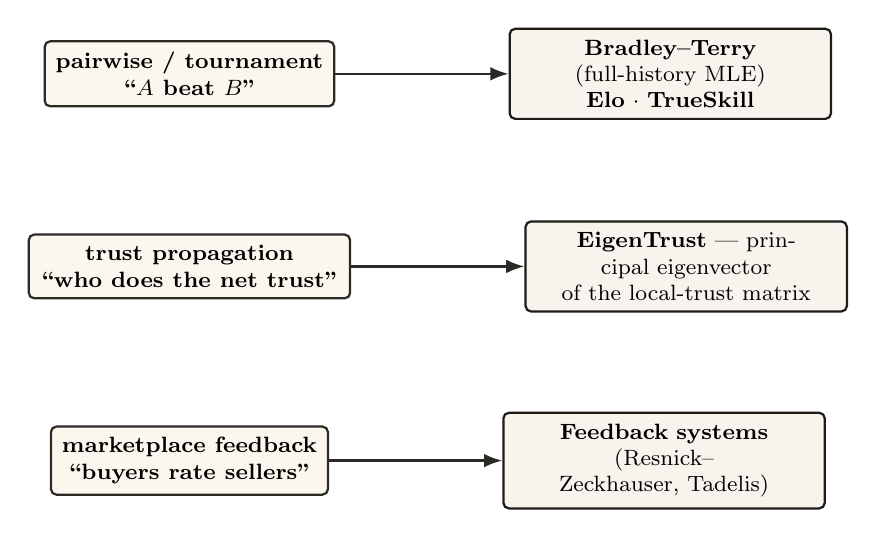
\begin{tikzpicture}[
  font=\small,
  sig/.style={draw=hhink,thick,fill=hhpaper,rounded corners=2pt,inner sep=4pt,
              align=center,minimum width=34mm,font=\bfseries\footnotesize},
  est/.style={draw=hhebony,thick,fill=hhsand!30,rounded corners=2pt,inner sep=4pt,
              align=center,minimum width=40mm,text width=38mm,font=\footnotesize},
  arr/.style={->,>=Latex,thick,draw=hhink},
]

\node[sig] (s1) at (0,2) {pairwise / tournament\\``$A$ beat $B$''};
\node[sig,below=16mm of s1] (s2) {trust propagation\\``who does the net trust''};
\node[sig,below=16mm of s2] (s3) {marketplace feedback\\``buyers rate sellers''};

\node[est,right=22mm of s1] (e1)
  {\textbf{Bradley--Terry} (full-history MLE)\\ \textbf{Elo} $\cdot$ \textbf{TrueSkill}};
\node[est,right=22mm of s2] (e2)
  {\textbf{EigenTrust} --- principal eigenvector\\ of the local-trust matrix};
\node[est,right=22mm of s3] (e3)
  {\textbf{Feedback systems}\\ (Resnick--Zeckhauser, Tadelis)};

\draw[arr] (s1) -- (e1);
\draw[arr] (s2) -- (e2);
\draw[arr] (s3) -- (e3);


\end{tikzpicture}}
\caption{\textbf{The estimator family, by signal type} --- the wrong choice is a
real error. Pairwise outcomes call for Bradley--Terry / Elo / TrueSkill; network
trust calls for EigenTrust (PageRank for reputation --- \emph{not} a bandit);
marketplace feedback calls for feedback systems with measured price premia
(Resnick--Zeckhauser's ${\sim}8\%$; Tadelis on adverse selection). A SQLite harbor holds the \emph{whole} settled-outcome
history, so it is in the Bradley--Terry regime, not the streaming-Elo regime. None
of these is the hard part: the estimator is \emph{cheap and last}, while the
substrate beneath --- non-forgeable identity, continuity, an oracle-witnessed
ledger --- is the gate.}
\label{fig:estimators}
\end{figure}


\subsection{Score as telemetry; gate on predicates}

\keyidea{Publish the score as \emph{telemetry} (a signal the operator and the
buyer can read), but \emph{gate} on \emph{predicates} (machine-checkable witnessed
facts: ``passed the acceptance test,'' ``no slashed bond in the last $k$
settlements''). The instant the score itself becomes the gate, it becomes a
Goodhart target~\cite{strathern1997}: ``when a measure becomes a target it ceases
to be a good measure.''}

\begin{exercises}
\textit{Check.} (1) Why is a SQLite harbor in the Bradley--Terry regime rather
than the streaming-Elo regime? \\
\textit{Trace.} (2) You have one task with a clear binary acceptance test, and
another judged only by a human's aesthetic preference. Which estimator fits each,
and why does EigenTrust fit neither directly? \\
$\star$ \textit{Open.} (3) The substrate-vs-score sentence says the estimator is
``cheap and last.'' Construct a scenario where a \emph{better estimator} still
buys nothing because the substrate is rotten (e.g.\ forgeable identity or an
agent-authored oracle). Generalize the lesson.
\end{exercises}

% ═════════════════════════════════════════════════════════════════════════════
\section{Why reputation is \emph{not} a bandit problem}\label{sec:not-bandit}
% ═════════════════════════════════════════════════════════════════════════════

It is tempting --- and the routing literature invites the temptation --- to model
``which agent/model/skill should I pick?'' as a \textbf{multi-armed
bandit}~\cite{lattimore2020bandit}: arms are agents, pulling an arm yields a
reward, and Thompson sampling~\cite{thompson1933} or UCB balances exploration
against exploitation. That framing is correct for one narrow internal task and
catastrophically wrong for reputation as a whole. The distinction is load-bearing
enough to state as a claim.

\pullquote{\emph{Internal routing} --- one operator privately choosing which of
their own agents to spawn next --- is bandit-shaped. \emph{Reputation} --- a public,
adversarial, multi-dimensional, persistent substrate other parties trade on --- is
not. Modeling reputation as a bandit imports four assumptions that are all false in
a market.}

% --- FIGURE 9: bandit assumptions vs reputation reality ---
% Fig 9 — bandit assumptions vs reputation reality (the four breaks).
\providecolor{hhsand}{HTML}{E9DCC4}
\providecolor{hhsanddeep}{HTML}{D8C7A6}
\providecolor{hhebony}{HTML}{121212}
\providecolor{hhink}{HTML}{1B1712}
\providecolor{hhcobalt}{HTML}{003FB8}
\providecolor{hhamber}{HTML}{6B4500}
\providecolor{hhteal}{HTML}{00564C}
\providecolor{hhpaper}{HTML}{FBF7EF}

\begin{figure}[H]
\centering
\small
\renewcommand{\arraystretch}{1.4}
\begin{tabular}{@{}p{4.2cm} p{5.0cm} p{5.4cm}@{}}
\toprule
\textbf{Bandit assumes\ldots} & \textbf{\ldots but reputation is\ldots} & \textbf{The right tool instead} \\
\midrule
\textcolor{hhteal}{\textbf{Stationary}} arm rewards &
  \textcolor{hhcobalt}{\textbf{non-stationary}}: models upgrade, skills version,
  reputation bubbles build \& collapse (Liu--Skrzypacz) &
  bounded-memory reputation dynamics; version-binding \\
\textcolor{hhteal}{\textbf{One scalar}} reward &
  \textcolor{hhcobalt}{\textbf{multi-dimensional}}: accuracy / aesthetics /
  efficiency, in tension, buyer-weighted &
  a quality \emph{vector} + buyer preference (\S\ref{sec:adr0049}) \\
\textcolor{hhteal}{\textbf{Non-strategic}} environment &
  \textcolor{hhcobalt}{\textbf{strategically adversarial}}: Goodhart,
  wash-trading, whitewashing, collusion &
  mechanism design (Nisan et al.), bonds \& slashing \\
\textcolor{hhteal}{\textbf{Observed}} reward signal &
  \textcolor{hhcobalt}{\textbf{produced by a capturable oracle}} with its own
  incentives &
  bond-and-slash judges; rate-the-raters ($\S$\ref{sec:oracle}) \\
\bottomrule
\end{tabular}

\vspace{4pt}
\centering
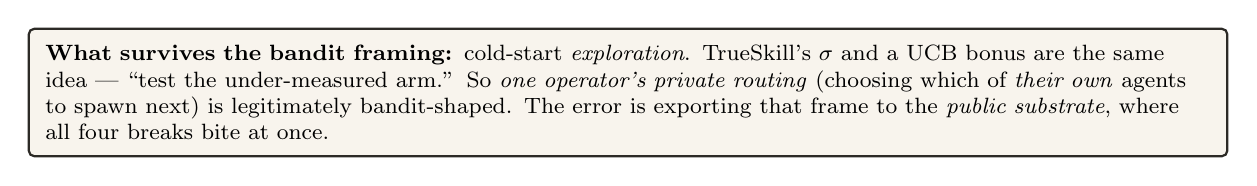
\begin{tikzpicture}
\node[draw=hhink,thick,fill=hhsand!30,rounded corners=2pt,inner sep=6pt,
      text width=148mm,align=left,font=\footnotesize] {%
  \textbf{What survives the bandit framing:} cold-start \emph{exploration}.
  TrueSkill's $\sigma$ and a UCB bonus are the same idea --- ``test the
  under-measured arm.'' So \emph{one operator's private routing} (choosing which of
  \emph{their own} agents to spawn next) is legitimately bandit-shaped. The error is
  exporting that frame to the \emph{public substrate}, where all four breaks bite at
  once.};
\end{tikzpicture}
\caption{\textbf{Why reputation is not a bandit problem.} A multi-armed bandit
imports four assumptions --- stationarity, a scalar reward, a non-strategic
environment, and an observed reward signal --- all false for a public reputation
substrate. Exploration (one operator's private routing) is the one place the bandit
framing legitimately survives.}
\label{fig:not-bandit}
\end{figure}


\subsection{The four broken assumptions}

\begin{enumerate}[leftmargin=1.6em]
  \item \textbf{Stationarity.} Bandit regret bounds assume the reward
  distribution of each arm is (near-)stationary. Agent quality is
  \emph{non-stationary} by construction: models are upgraded, skills are versioned,
  prompts drift, and a skill's reputation built on v1 says nothing about v2. The
  Liu--Skrzypacz line of work on \emph{reputation
  bubbles}~\cite{liuskrzypacz2014} shows that with bounded memory and
  non-stationary types, reputation can build and \emph{collapse} in cycles ---
  behavior a stationary-arm bandit cannot represent.
  \item \textbf{One scalar reward.} A bandit optimizes a single scalar. Quality is
  \emph{multi-dimensional}: accuracy, aesthetics, and efficiency are different
  axes, often in tension (the fast cheap answer is rarely the most beautiful), and
  a buyer's weighting of them is a \emph{preference vector}, not a constant. Collapse
  them into one scalar and you have re-created the Goodhart target the substrate
  argument warned against (\S\ref{sec:adr0049}).
  \item \textbf{A non-strategic environment.} Bandit arms do not \emph{try} to
  look good. Agents and their principals are \emph{strategic adversaries}: they
  will Goodhart the measured axis, wash-trade fake outcomes, whitewash a bad
  record, and collude. A reputation mechanism is a \emph{game}, and the relevant
  tool is mechanism design~\cite{nisan2007agt}, not regret minimization.
  \item \textbf{A trusted reward signal.} The deepest break: a bandit
  \emph{observes} its reward. In a market, the reward (the grade) is
  \emph{produced} by an evaluator who has their own incentives. The grading
  oracle's incentive-compatibility is not a side-issue --- it is a hole in the core
  theorem (\S\ref{sec:oracle}). A bandit framing simply assumes the hole away.
\end{enumerate}

\subsection{What survives the bandit framing}

To be fair to the bandit literature: cold-start \emph{exploration} is real, and the
right place to borrow from bandits is the \emph{exploration bonus}. TrueSkill's
$\sigma$ and a UCB-style bonus are the same idea --- ``test the under-measured
arm.'' So \emph{within one operator's private routing}, a contextual bandit
conditioned on the operator's cost/quality preference vector is a fine engineering
choice. The error is exporting that frame to the \emph{public substrate}, where
non-stationarity, multi-dimensionality, strategy, and an untrusted reward signal
all bite at once.

\pitfall{``We'll just run Thompson sampling over the agents'' is the most common
way an agent-economy design quietly assumes its hardest problems away. It assumes a
trusted reward (no judge-capture), a scalar reward (no aesthetics-vs-efficiency
tension), a non-strategic environment (no Goodhart, no wash-trading), and
stationarity (no model upgrades). All four are false in a market.}

\begin{exercises}
\textit{Check.} (1) Name the four bandit assumptions and the market reality that
breaks each. \\
\textit{Trace.} (2) Identify the \emph{one} place a bandit \emph{is} the right
tool in this paper, and explain why it survives the four objections there. \\
$\star$ \textit{Open.} (3) Chiu--Zhang--van der Schaar~\cite{chiu2025strategic}
show competitive agents over-invest in self-improvement, burning surplus despite
individual rationality. Does capping the reputation signal's marginal return
restore efficiency, or merely relocate the waste? This is the self-improvement
arms-race open problem.
\end{exercises}

% ═════════════════════════════════════════════════════════════════════════════
\section{ADR-0049: multi-dimensional reputation and neutral judges}\label{sec:adr0049}
% ═════════════════════════════════════════════════════════════════════════════

We now design, in this paper, the architecture the volume calls \textbf{ADR-0049}.
It has three parts: a multi-dimensional quality vector; a market of neutral,
conflict-free, influence-free evaluators; and a skill$\to$agent helpfulness
attribution. We state it as a design (\DESIGNED-to-\VISION), honestly: no
\verb|lib/reputation.ts| exists yet.

\subsection{Multi-dimensional quality (different axes, different judges)}

\begin{definition}[Quality vector]\label{def:qvec}
A witnessed outcome carries a \textbf{quality vector}
$\mathbf{q} = (q_{\text{acc}}, q_{\text{aes}}, q_{\text{eff}})$ over the axes
\emph{accuracy} (did it do the right thing, against an oracle), \emph{aesthetics}
(is the artifact good --- code clarity, design taste --- judged by an expert), and
\emph{efficiency} (tokens, wall-clock, dollars, from the cost ledger
\verb|lib/cost-ledger.ts|, \BUILT). Each axis is scored by a \emph{different judge},
because the competent judge of accuracy (a test oracle) is not the competent judge
of aesthetics (a senior reviewer) is not the competent judge of efficiency (a
meter).
\end{definition}

\noindent The buyer reads the \emph{vector} and applies their own weighting (the
operator's ``cheap vs.\ careful'' preference). Publishing a vector and letting the
buyer weight it is the natural disclosure form --- and it is precisely what avoids
re-collapsing quality into one Goodhart-able scalar. The open design question of
\emph{whether} a vector disclosure lets agents Goodhart the most-weighted axis is
named as a starred exercise.

% --- FIGURE 10: the multi-dimensional reputation vector ---
% Reader question: how does quality differ across dimensions rather than
% collapse to one score? Claim: the same two outcome vectors legitimately
% reverse rank once independent judges disclose per-axis scores and a buyer
% applies its own weights -- no premature averaging is needed to explain the
% reversal. Evidence: outcome A=(1,.85,.45), outcome B=(.75,.55,1) on
% accuracy/aesthetics/efficiency, each independently judged; a security buyer
% (weights .60,.30,.10) selects A, a cost buyer (weights .15,.15,.70) selects
% B. Must distinguish: the three independently judged axes from a single
% averaged score, and which buyer selects which outcome. Grammar: an aligned
% dot profile across three axes plus a buyer-selection strip, rejected: a
% radar chart (area exaggerates the axis with the largest scale) and a single
% average badge (hides the exact reversal this figure exists to show).
% Five-second test: a reader says "same two vectors, opposite winners."
\begin{figure}[H]
\centering
\pdfigurehue{pdviolet}%
\begin{tikzpicture}[pd figure,x=.95cm,y=1cm]
  \node[pd title,anchor=west] at (0,3.9) {witnessed outcome profiles remain vectors};
  % ---- three independently judged axes --------------------------------------
  \foreach \x/\axis/\judge in {0.75/accuracy/test oracle,3.55/aesthetics/expert reviewer,6.35/efficiency/cost ledger} {
    \draw[pd hairline] (\x,0) -- (\x,2.60);
    \foreach \y in {0,.65,1.30,1.95,2.60} \draw[pd tick] ({\x-.11},\y) -- ({\x+.11},\y);
    \node[pd title,anchor=north] at (\x,-.20) {\axis};
    \node[pd note,anchor=north] at (\x,-.56) {\judge};
  }
  % A=(1,.85,.45), B=(.75,.55,1), scaled to the 0..2.60 axis
  \draw[pd focus rule,line width=1.5pt] (0.75,2.60) -- (3.55,2.21) -- (6.35,1.17);
  \draw[pd breach rule,dashed,line width=1.5pt] (0.75,1.95) -- (3.55,1.43) -- (6.35,2.60);
  \foreach \x/\y in {0.75/2.60,3.55/2.21,6.35/1.17} \node[pd focus datum] at (\x,\y) {};
  \foreach \x/\y in {0.75/1.95,3.55/1.43,6.35/2.60} \node[pd breach datum] at (\x,\y) {};
  \node[pd focus label,anchor=north east] at (6.1,1.0) {outcome A};
  \node[pd breach label,anchor=south east] at (6.1,2.75) {outcome B};
  % ---- buyers apply preferences after disclosure -----------------------------
  \node[pd title,anchor=west] at (0,-1.55) {buyers apply preferences after disclosure};
  \draw[pd hairline] (0,-2.55) -- (6.50,-2.55);
  \draw[pd hairline] (0,-3.45) -- (6.50,-3.45);
  \node[pd title,anchor=east] at (-.20,-2.55) {security buyer};
  \node[pd note,anchor=east] at (-.20,-2.90) {weights $.60,.30,.10$};
  \node[pd title,anchor=east] at (-.20,-3.45) {cost buyer};
  \node[pd note,anchor=east] at (-.20,-3.80) {weights $.15,.15,.70$};
  \node[pd focus datum] at (4.55,-2.55) {};
  \node[pd breach datum] at (2.10,-2.55) {};
  \node[pd focus datum] at (0.85,-3.45) {};
  \node[pd breach datum] at (4.45,-3.45) {};
  \node[pd focus label,anchor=south west] at (4.75,-2.45) {A selected};
  \node[pd breach label,anchor=south west] at (4.65,-3.35) {B selected};
  \node[pd label,anchor=north] at (0,-4.05) {lower weighted fit};
  \node[pd label,anchor=north] at (6.50,-4.05) {higher weighted fit};
\end{tikzpicture}
\caption{A favours accuracy and aesthetics; B favours efficiency. Different buyer priorities legitimately reverse the ranking. A universal average would erase that choice. [internal]}
\label{fig:multidim}
\end{figure}


\subsection{The neutral-judge market (the harbor's universities and rating agencies)}

A judge that grades the work of a party it has a stake in is not a judge. The
metaphor the volume uses is exact: a reputation needs the equivalent of
\emph{universities} (which certify competence) and \emph{rating agencies} (which
rate counterparties) --- third parties whose value is precisely that they are
\emph{neutral}. We make ``neutral'' a checklist, not a vibe:

\begin{itemize}[leftmargin=1.4em]
  \item \textbf{Conflict-free.} The judge has no bond, stake, or principal-link in
  the work being graded. (Excludes self-grading and same-principal grading.)
  \item \textbf{Influence-free.} The judge cannot be paid \emph{by the graded
  party} for a better grade. Funding is the hard part: a paid judge has a client,
  an unpaid judge does not scale. The resolution (\S\ref{sec:oracle}) is that
  judges post their \emph{own} bond and carry their \emph{own} reputation.
  \item \textbf{De-biased, for LLM judges.} An LLM-as-judge~\cite{zheng2023judging}
  carries position, verbosity, and \emph{self-enhancement} bias (a backend rates
  its own family up). The discipline is blind, order-swap, pairwise, and
  family-exclude scoring --- never let a backend judge its own family unblinded.
\end{itemize}

\noindent Crucially, an expert third-party judge is \emph{hired through Port
Daddy's own protocols}: judging is itself a float-planned, bonded task
(Paper~4's escrow ceremony), so the harbor that runs the market also runs the
hiring of the judges who keep it honest. Figure~\ref{fig:judge-market} draws this:
the graded work flows to a judge selected for conflict-/influence-freedom, the
judge posts a bond, the grade enters the outcome ledger, and a later re-audit can
slash a judge whose grade is overturned.

% --- FIGURE 11: the neutral-judge market ---
% Reader question: how is a neutral judge selected, informed, and paid?
% Claim: the judge market has two different proof moments -- neutrality is
% earned before selection (visible exclusion, then a public draw), and
% accountability is an exposure interval after it (a bond that stays at risk
% through the dispute window, not a one-time label). Evidence: six candidates,
% three excluded for a principal/stake/model-family conflict with the graded
% party, a public draw from the remaining three, then submit/filter/select/
% blind grade/ledger/re-audit, with the bond exposed from select through
% re-audit. Must distinguish: the exclusion step (before) from the bond
% exposure interval (after); the slash consequence from the re-audit step
% itself. Grammar: an actor pool with a filter, feeding a step rail with an
% exposure interval underneath, rejected: a marketplace network graph (no
% order, no exposure) and a central judge circle (implies a chosen identity
% carries neutrality, not the checkable history). Five-second test: a reader
% says "excluded before the draw; exposed after it, until re-audit."
\begin{figure}[H]
\centering
\pdfigurehue{pdviolet}%
\begin{tikzpicture}[pd figure,x=1cm,y=1cm]
  \node[pd title,anchor=west] at (0,7.90) {eligibility is established before the grade};
  % ---- candidate pool and explicit exclusions --------------------------------
  \foreach \x/\lab in {1.0/$J_1$,2.3/$J_2$,3.6/$J_3$,4.9/$J_4$,6.2/$J_5$,7.5/$J_6$}
    \node[pd state,circle,minimum size=7.5mm,inner sep=0pt] (\lab) at (\x,6.60) {\lab};
  \foreach \x in {1.0,3.6,7.5} {
    \draw[pd breach rule] ({\x+.16},6.76) -- ({\x+.40},7.00);
    \draw[pd breach rule] ({\x+.16},7.00) -- ({\x+.40},6.76);
  }
  \node[pd breach label,anchor=west,text width=2.5cm] at (7.95,6.60)
    {excluded: shares a principal, stake, or model family with the graded party};
  % ---- funnel remaining candidates to a public selection point --------------
  \foreach \x in {2.3,4.9,6.2} \draw[pd hairline] (\x,6.18) -- (4.9,5.30);
  \node[pd focus datum] (draw) at (4.9,5.05) {};
  \node[pd focus label,anchor=west] at (5.15,5.05) {public draw from eligible pool};
  % ---- ceremony rail, steps named above it -----------------------------------
  \draw[pd rule,-{Stealth[length=1.8mm,width=1.1mm]}] (0.6,3.30) -- (10.6,3.30);
  \foreach \x/\lab in {1.3/submit,3.0/filter,4.9/select,6.6/{blind grade},8.3/ledger,9.9/{re-audit}} {
    \draw[pd tick] (\x,3.15) -- (\x,3.45);
    \node[pd label,anchor=south,align=center,text width=1.55cm] at (\x,3.55) {\lab};
  }
  \node[pd focus datum] at (3.0,3.30) {};
  \node[pd focus datum] at (4.9,3.30) {};
  \node[pd focus datum] at (6.6,3.30) {};
  \node[pd focus datum] at (8.3,3.30) {};
  \node[pd breach datum] at (9.9,3.30) {};
  % ---- bond exposure is an interval, not a one-time label --------------------
  \draw[pd breach rule,line width=1.45pt] (4.9,0.90) -- (9.9,0.90);
  \node[pd breach datum] at (4.9,0.90) {};
  \node[pd breach datum] at (9.9,0.90) {};
  \node[pd breach label,anchor=south east,text width=4.0cm,align=right] at (6.9,1.15)
    {judge bond remains exposed through the dispute window};
  \draw[pd breach arrow] (9.9,3.05) -- (9.9,1.15);
  \node[pd breach label,anchor=east,text width=1.9cm,align=right] at (9.65,2.45) {slash if overturned};
  % ---- the ledger: every step is one inspectable history ---------------------
  \draw[pd focus rule] (1.3,-0.20) -- (8.3,-0.20);
  \node[pd focus label,anchor=north,text width=9.0cm,align=center] at (4.8,-0.40)
    {receipt, exclusions, selection, grade, and audit remain one inspectable history};
\end{tikzpicture}
\caption{Before selection, exclusions and a public draw support neutrality. After selection, a bond and later re-audit support accountability. Both stages leave checkable evidence. [internal]}
\label{fig:judge-market}
\end{figure}


\subsection{Skill $\to$ agent helpfulness attribution}

A distinctive, tractable, and \emph{shippable-soon} signal: track whether a
\textbf{skill} (a \verb|SKILL.md|, its referenced docs, or its scripts ---
\verb|skills/*/SKILL.md|) actually \emph{helped} an agent, \emph{especially when
that skill's content was loaded into the agent's context window}. The witnessed
event is concrete: skill $s$ was grafted into agent $a$'s context at task $t$;
$t$ later settled with quality vector $\mathbf{q}$. Over many such events we
estimate a \emph{skill-helpfulness} effect --- did loading $s$ raise $\mathbf{q}$
relative to comparable tasks without it? This is reputation for \emph{tools},
keyed on witnessed, context-attributable outcomes, and it is the licensing side's
substrate (Paper~4). It is also the cleanest near-term instance of the whole
thesis: a non-forgeable event (the graft), a witnessed outcome (the settled task),
and a multi-dimensional grade --- no bandit required.

\pitfall{Attribution is not causation. ``Skill $s$ was in context and the task
succeeded'' does not prove $s$ caused the success. The honest estimate needs a
comparison set (similar tasks without $s$) and is still observational. Sell it as
\emph{helpfulness evidence}, not \emph{proof of value}, and gate licensing
clawbacks on the witnessed green/red settlement, not on the helpfulness estimate
alone.}

\begin{exercises}
\textit{Check.} (1) For each of accuracy / aesthetics / efficiency, name a
competent judge and an \emph{incompetent} one. \\
\textit{Trace.} (2) Walk a judging task through Port Daddy's bonded protocol: who
float-plans it, who posts the bond, where does the grade land, and what slashes the
judge? \\
\textit{Trace.} (3) Design the witnessed event for skill-helpfulness. What fields
does it need so that a buyer can verify ``this skill helped'' without trusting the
skill's author? \\
$\star$ \textit{Open.} (5) If you publish the 3-vector and buyers weight it, do
agents Goodhart the most-weighted axis? If you publish a scalar, you have recreated
the bandit framing the substrate argument rejects. What is the right disclosure
form for vector reputation?
\end{exercises}

% ═════════════════════════════════════════════════════════════════════════════
\section{The grading oracle's incentive-compatibility}\label{sec:oracle}
% ═════════════════════════════════════════════════════════════════════════════

Every folk-theorem incentive-compatibility result in the L3 economy bottoms out in
``the daemon derives the grade'' --- but the grade is produced by a
\emph{capturable evaluator}. This is not a side-gap. It is a hole in the
\emph{core theorem}, and we treat it head-on rather than assuming it away.

\begin{property}[The grading-oracle hole]\label{prop:hole}
Let an outcome's settlement (and thus the bond flow and the reputation update)
depend on a grade $g$ produced by an evaluator $J$. If $J$ can be captured ---
bribed, colluded with, or self-interested --- then the incentive-compatibility of
\emph{every} mechanism that settles on $g$ is only as strong as $J$'s own honesty.
Assuming $J$ honest is assuming the conclusion.
\end{property}

\noindent There are two honest ways to close the hole, and a recursion to bound.

\paragraph{Option A --- bond-and-slash the judges.}
Make judging a bonded role (\S\ref{sec:adr0049}): $J$ posts a bond before grading;
a later \textbf{re-audit} (a fresh, conflict-free judge, sampled) that overturns
$J$'s grade \emph{slashes} $J$. Now lying has an expected cost, and a judge's own
reputation is the asset they protect. This converts ``trust the oracle'' into
``the oracle has skin in the game,'' which is the same move slashing makes for
agents.

\paragraph{Option B --- 2-of-3 multi-oracle.}
Settle disputes against a quorum of independent oracles (automated test / evidence
review / human), so capturing the grade requires capturing a majority. This raises
the cost of capture but does not eliminate it, and the \emph{human} oracle is a
scarce, expensive, capturable resource in its own right (the economics of
arbitration capacity is a named open problem, below).

\paragraph{The rate-the-raters recursion --- does it terminate?}
Option~A pushes the problem up a level: who audits the auditors? The re-auditor is
itself a judge with incentives. The recursion ``rate the raters who rate the
raters'' must be shown to \emph{terminate} or to \emph{contract}. We do not claim a
proof; we claim the shape of one and mark the rest open.

% --- FIGURE 12: rate-the-raters recursion ---
% Audit tower for Sec. stp-rate-the-raters ("Numbers by hand": the audit tower).
% Small multiples on one shared audit-level axis, so the three closing depths are
% read as three lengths on a common scale. Every point is the chapter's own
% two-phase recurrence at the chapter's own parameters -- G_0 = 400, B = 50,
% rho*d = 0.2, beta = rho*d*B = 10: while G_k > C*B bribing all C cliques still
% pays and value bleeds LINEARLY by C*beta per level; below that threshold it
% decays GEOMETRICALLY by lambda = 1-rho*d = 0.8. The three depths (27, 36, 53)
% and the three bond totals ($1,350 / $1,800 / $2,650) are the chapter's own.
% Every region carries an explicit drawn edge because the Swiss edition's
% pd caution fill override sets draw=none.
% Data: whitepaper/figures/data/audit-tower-depth.csv, emitted by
% whitepaper/figures/data/make-figure-data.py (deterministic, no seed) [verified].
\begin{figure}[H]
\centering
\pgfplotsset{
  every axis/.append style={
    width=8.55cm,height=2.30cm,
    axis lines=left,
    ymode=log,log basis y=10,
    xmin=0,xmax=57,ymin=0.7,ymax=560,
    ytick={1,10,100},yticklabels={1,10,100},
    xlabel={},ylabel={},
    tick label style={font=\footnotesize,text=hhgray},
    axis line style={draw=hhgray,line width=.45pt},
    tick style={draw=hhgray,line width=.45pt},
    scale only axis,
    clip=false,
  }}
\begin{tikzpicture}[pd figure]

  % ---------------- C = 8: heterogeneous, geometric from level 0 --------------
  \begin{axis}[name=top,xtick=\empty,anchor=north west,at={(0cm,0cm)}]
    \addplot[draw=hhink,line width=.62pt,forget plot,domain=0:57,samples=2]{1};
    \addplot[draw=hhteal,line width=1.15pt,forget plot]
      coordinates {(0,400) (1,320) (2,256) (3,204.8) (4,163.8) (6,104.9) (8,67.11)
        (10,42.95) (12,27.49) (14,17.59) (16,11.26) (18,7.206) (20,4.612)
        (22,2.951) (24,1.889) (26,1.209) (27,0.967)};
    \node[pd focus datum] at (axis cs:27,0.967) {};
    \node[pd direct label,text=hhteal,anchor=west] at (axis cs:29,2.4)
      {closes at 27 levels, \$1,350};
    \node[pd row label,anchor=north east] at (axis cs:56.5,320)
      {eight cliques};
    \node[pd direct label,text=hhteal,anchor=west] at (axis cs:2.2,2.0)
      {no bribery phase};
  \end{axis}

  % ---------------- C = 2: 15 levels of bribery, then geometric ---------------
  \begin{axis}[name=mid,xtick=\empty,anchor=north west,at={(0cm,-2.72cm)}]
    \addplot[pd caution fill,draw=hhamber!75,line width=.4pt,forget plot]
      coordinates {(0,0.7) (15,0.7) (15,560) (0,560)} \closedcycle;
    \addplot[draw=hhink,line width=.62pt,forget plot,domain=0:57,samples=2]{1};
    \addplot[draw=hhink,line width=1.0pt,forget plot]
      coordinates {(0,400) (1,380) (2,360) (3,340) (4,320) (6,280) (8,240)
        (10,200) (12,160) (14,120) (15,100) (16,80) (18,51.2) (20,32.77)
        (22,20.97) (24,13.42) (26,8.59) (28,5.498) (30,3.518) (32,2.252)
        (34,1.441) (36,0.9219)};
    \node[pd focus datum] at (axis cs:36,0.9219) {};
    \node[pd direct label,anchor=west] at (axis cs:38,2.4) {36 levels, \$1,800};
    \node[pd row label,anchor=north east] at (axis cs:56.5,320) {two cliques};
    \node[pd direct label,text=hhamber,anchor=west] at (axis cs:1.0,4.0)
      {bribery phase};
  \end{axis}

  % ---------------- C = 1: 35 levels of bribery, then geometric ---------------
  \begin{axis}[name=bot,anchor=north west,at={(0cm,-5.44cm)},
      xtick={0,10,20,27,36,53},
      xlabel={audit level $k$ \ (one bond $B=50$ posted per level)},
      xlabel style={font=\footnotesize,text=hhgray}]
    \addplot[pd caution fill,draw=hhamber!75,line width=.4pt,forget plot]
      coordinates {(0,0.7) (35,0.7) (35,560) (0,560)} \closedcycle;
    \addplot[draw=hhink,line width=.62pt,forget plot,domain=0:57,samples=2]{1};
    \addplot[draw=hhamber,line width=1.15pt,dash pattern=on 3pt off 2pt,forget plot]
      coordinates {(0,400) (2,380) (4,360) (6,340) (8,320) (10,300) (12,280)
        (14,260) (16,240) (18,220) (20,200) (22,180) (24,160) (26,140) (28,120)
        (30,100) (32,80) (34,60) (35,50) (36,40) (38,25.6) (40,16.38) (42,10.49)
        (44,6.711) (46,4.295) (48,2.749) (50,1.759) (52,1.126) (53,0.9008)};
    \node[pd focus datum] at (axis cs:53,0.9008) {};
    \node[pd direct label,text=hhamber,anchor=east] at (axis cs:56.5,45)
      {53 levels, \$2,650};
    \node[pd direct label,text=hhamber,anchor=west] at (axis cs:1.0,4.0)
      {bribery phase};
    \node[pd row label,anchor=north east] at (axis cs:56.5,320) {one clique};
  \end{axis}

  \node[pd axis label,rotate=90,anchor=south] at (-1.35,-3.85)
    {surviving corrupt value $G_k$};
\end{tikzpicture}
\caption{\textbf{A recursive audit closes at a depth set by how the judge pool is
sampled, not by how tall the tower is drawn.} Surviving corrupt value against
audit level, one panel per clique count, on one shared level axis, at the
chapter's running parameters $G_0=400$, $B=50$, $\rho d=0.2$, so $\beta=\rho
dB=10$ and $\lambda=1-\rho d=0.8$. Bribing all $C$ cliques pays while $G_k>CB$,
and in that shaded phase value bleeds \emph{linearly} by $C\beta$ per level;
only past it does it contract geometrically, which on a log axis is the straight
stretch. A heterogeneous pool at $C=8$ has no bribery phase at all
($CB=400\not<G_0$) and closes in $27$ levels for \$1,350; two cliques bleed for
$15$ levels first and need $36$ for \$1,800; a monoculture bleeds for $35$ and
needs $53$ for \$2,650. Buying cliques is worth more than buying bond. The
contraction bounds the tower; it does not supply the exogenously honest root the
tower terminates in, nor the telemetry that estimates $d$. [verified against the
chapter's own arithmetic; \texttt{figures/data/audit-tower-depth.csv} from
\texttt{figures/data/make-figure-data.py}, deterministic]}
\label{fig:rate-raters}
\end{figure}


\begin{conjecture}[Contractive re-audit]\label{conj:contract}
If (i) re-audits are sampled with probability $\rho$, (ii) an overturned grade
slashes a bond $B_J$ strictly exceeding the maximum bribe a single graded party
can offer, and (iii) re-auditors are themselves drawn conflict-free from a pool
larger than any single colluding clique, then the expected gain from dishonest
grading is negative at \emph{every} level of the recursion, and the
``rate-the-raters'' tower is \emph{contractive}: the incentive to corrupt level
$k+1$ is strictly smaller than at level $k$, so the tower has a finite honest
fixed point.
\end{conjecture}

\pitfall{Conjecture~\ref{conj:contract} is \emph{conjectured}, not proven. It is
the precise statement of what Paper~4's central incentive-compatibility result
\emph{needs} and currently \emph{lacks}. The contribution here is to name the hole
exactly, give two candidate closures, and state the termination obligation ---
\emph{not} to claim it is closed. Honest labels apply: this is \VISION.}

\keyidea{The grading oracle is the load-bearing assumption hidden under every IC
claim in the economy. ``The daemon derives the grade'' only helps if the grade's
\emph{producer} is itself incentive-compatible. Either bond-and-slash the judges
and prove the rate-the-raters recursion contracts, or accept that the core theorem
is conditional on an honest oracle --- and say which.}

\begin{exercises}
\textit{Check.} (1) State Property~\ref{prop:hole} and explain why ``the daemon
derives the grade'' does not, by itself, close it. \\
\textit{Trace.} (2) Walk Option~A: a judge grades dishonestly, a re-audit
overturns it. Follow the bond flow and the reputation update for the judge. \\
$\star$ \textit{Open.} (4) Prove or refute Conjecture~\ref{conj:contract}. If the
re-audit probability $\rho$ is too low, the tower is not contractive --- find the
critical $\rho^\star$ as a function of bond size and bribe ceiling. \\
$\star$ \textit{Open.} (10) Arbitration capacity: human oracles are scarce. Design
a market for bonded, rated, slashable arbiters and argue whether it converges to
honest rulings or to rubber-stamping under load.
\end{exercises}

% ═════════════════════════════════════════════════════════════════════════════
\section{Revocation, tombstones, and bounded memory}\label{sec:revoke}
% ═════════════════════════════════════════════════════════════════════════════

A reputation built on witnessed outcomes must answer two questions the cheerful
``reputation never ends'' framing dodges: what happens when a witnessed outcome
turns out to be \emph{fraudulent}, and is no-decay actually \emph{good}? We adopt
the volume's reconciled position on both, against the naive version.

\subsection{Monotone in honest outcomes, individually revocable}

\begin{property}[Reputation monotonicity with tombstones]\label{prop:tombstone}
Reputation is \textbf{monotone in \emph{honest} witnessed outcomes} --- a genuine
delivery is never silently erased by the passage of time --- \emph{but} a witnessed
outcome is itself \textbf{individually revocable via a propagating tombstone}: a
compensating, append-only entry that retracts a specific outcome later found
fraudulent (a colluding judge, a faked oracle). ``Never decays'' applies to honest
outcomes \emph{only}; it is \emph{not} an anti-revocation property.
\end{property}

\noindent This is a \textbf{saga}-style compensation~\cite{garcia1987sagas}: you do
not mutate the ledger in place (that would break append-only and auditability);
you append a tombstone that nullifies the targeted entry, and the tombstone
\emph{propagates} across harbors bounded by the federation's revocation-convergence
window (Paper~4). The poisoned data point was spendable only during the propagation
window; bounding that window is the federation's job.

% --- FIGURE 13: tombstone compensation on an append-only ledger ---
% Reader question: how does revoking an ancestor invalidate descendants
% without rewriting history? Claim: the append-only rail keeps every fact,
% including the fraud, forever inspectable; only the SEPARATE spendable-score
% trace changes, and it changes on a bounded delay, not instantly and not by
% deletion. Evidence: outcome o_3 (fraudulent), the overturning re-audit,
% tombstone t(o_3) appended, then imported at a foreign harbor; the fraud's
% contribution stays spendable until import, then falls to zero; the
% propagation window tau is measured, not asserted zero. Must distinguish:
% the append-only history (never mutated) from spendable score (the only
% thing that changes) and the bounded, not instantaneous, delay. Grammar:
% two aligned tracks on one time axis, an event rail above a step trace,
% rejected: cemetery/tombstone art (no mechanism) and a flat list of revoked
% IDs (no timing, no distinction between history and score). Five-second
% test: a reader says "the record never changes; only what it's worth does,
% and not instantly."
\begin{figure}[H]
\centering
\pdfigurehue{pdviolet}%
\begin{tikzpicture}[pd figure,x=1cm,y=1cm]
  \node[pd title,anchor=west] at (0,8.60) {append-only history};
  \draw[pd rule,-{Stealth[length=1.8mm,width=1.1mm]}] (0.65,7.20) -- (9.45,7.20);
  \foreach \x/\lab in {0.95/$o_1$,2.45/$o_2$,4.05/{$o_3$ fraudulent},5.65/{re-audit},
                       7.05/{$t(o_3)$ appended},8.80/{imported tombstone}} {
    \draw[pd tick] (\x,6.95) -- (\x,7.45);
    \node[pd label,anchor=south,align=center,text width=1.5cm] at (\x,7.60) {\lab};
  }
  \node[pd breach datum] at (4.05,7.20) {};
  \node[pd breach datum] at (7.05,7.20) {};
  \node[pd focus datum] at (8.80,7.20) {};
  \draw[pd breach rule] (3.75,6.90) -- (4.35,7.50);
  \draw[pd breach rule] (3.75,7.50) -- (4.35,6.90);
  \node[pd note,anchor=west,text width=9.3cm] at (0.65,6.30)
    {$o_3$ remains inspectable; $t(o_3)$ is a later compensating fact};
  % ---- contribution of o_3 to spendable reputation ---------------------------
  \node[pd title,anchor=west] at (0,4.55) {contribution of $o_3$ to spendable reputation};
  \draw[pd rule,-{Stealth[length=1.8mm,width=1.1mm]}] (0.65,-0.55) -- (9.45,-0.55);
  \draw[pd rule,-{Stealth[length=1.8mm,width=1.1mm]}] (0.65,-0.55) -- (0.65,3.10);
  \node[pd label,rotate=90,anchor=south,text width=3.4cm,align=center] at (-0.22,1.30) {score contribution};
  \draw[pd breach rule,line width=1.5pt]
    (0.65,-0.15) -- (4.05,-0.15) -- (4.05,1.60) -- (8.80,1.60);
  \draw[pd ready rule,line width=1.5pt] (8.80,1.60) -- (8.80,-0.15) -- (9.45,-0.15);
  \node[pd breach label,anchor=south west,text width=4.9cm] at (4.30,1.80)
    {fraud remains spendable while correction propagates};
  \node[pd ready label,anchor=south west] at (8.95,0.05) {nullified};
  \draw[pd breach rule,{Stealth[length=1.4mm,width=0.9mm]}-{Stealth[length=1.4mm,width=0.9mm]}] (7.05,-1.05) -- (8.80,-1.05);
  \node[pd breach label,anchor=north,text width=4.6cm,align=center] at (7.90,-1.25)
    {bounded propagation window $\tau$};
  \node[pd note,anchor=west,text width=9.3cm] at (0.65,-2.55)
    {the honest claim is a bounded window, not an instantaneous or history-deleting correction};
\end{tikzpicture}
\caption{\textbf{A tombstone changes score consumption without rewriting history.}
The upper rail remains append-only: fraudulent outcome $o_3$, the overturning
re-audit, and tombstone $t(o_3)$ are all preserved as distinct facts. The lower
trace shows what does change. The fraudulent contribution remains spendable until
the tombstone reaches an importing harbor, then falls to zero. The measured
interval $\tau$ is the federation's revocation-convergence obligation; the
protocol bounds that interval rather than pretending it never existed. [internal]}
\label{fig:tombstone}
\end{figure}


\subsection{Bounded memory is a design parameter, not a virtue to assert away}

The naive ``no decay window an agent can outrun'' framing sounds principled but is
mechanism-design-hostile. Liu--Skrzypacz~\cite{liuskrzypacz2014} show that with
\emph{bounded} memory, reputation can be welfare-\emph{improving} relative to
infinite memory --- and that infinite memory ($\infty$) is rarely optimal, because
it freezes types and removes the incentive to keep performing. Bounded memory is a
\textbf{tunable parameter}, and the right setting is an empirical/mechanism-design
question, not a slogan.

\pitfall{``Reputation never ends'' as a \emph{virtue} is wrong twice over: it
makes a fraudulent outcome permanent (needs the tombstone of
Property~\ref{prop:tombstone}), and it asserts $\infty$-memory is optimal when the
reputation-bubble literature shows it usually is not. Engage bounded memory as a
\emph{parameter}; do not assert no-decay as a feature.}

\keyidea{Two corrections to the cheerful framing: (1) reputation is monotone in
\emph{honest} outcomes but \emph{individually revocable} via a propagating
tombstone --- a saga compensation, not in-place mutation; (2) bounded memory is a
\emph{design parameter} (Liu--Skrzypacz reputation bubbles), not an anti-feature to
asser away.}

\begin{exercises}
\textit{Check.} (1) Why must revocation be a tombstone (append) rather than a
delete (mutate) on the outcome ledger? \\
\textit{Trace.} (2) A judge is later found to have colluded on five settled
outcomes. Walk the tombstone for one of them: what is appended, what propagates,
and what bounds the window the poisoned reputation was spendable? \\
$\star$ \textit{Open.} (8) Reputation-claim revocation with an append-only,
bounded-memory ledger across $N$ harbors: how do you prove the correction
converged and bound the spendable window, without violating append-only? This is
the cross-harbor analogue of capability revocation (Paper~4).
\end{exercises}

% ═════════════════════════════════════════════════════════════════════════════
\section{What this paper hands the market (Paper 4)}\label{sec:handoff}
% ═════════════════════════════════════════════════════════════════════════════

This paper is the bridge; its output is a precise hand-off to \emph{The Harbor
Economy} (Paper~4). We summarize what is delivered, what is borrowed, and what is
explicitly owed.

\begin{table}[H]
\centering
\small
\renewcommand{\arraystretch}{1.35}
\begin{tabular}{@{}p{5.2cm} p{2.0cm} p{7.2cm}@{}}
\toprule
\textbf{Artifact} & \textbf{Label} & \textbf{Role in Paper 4} \\
\midrule
Role / person distinction (Defs.~\ref{def:role}--\ref{def:person}) & --- &
The third side of the market is a \emph{tradeable person}, defined here. \\
Principal-as-economic-entity (Def.~\ref{def:principal}) & \DESIGNED &
Bonds and sanctions key on the principal; Paper~4 cross-references, not redefines. \\
The three continuity organs & \BUILT/\BUILTWEAK/\DESIGNED &
Reputation keys on organ~3 (the outcome ledger). \\
Outcome ledger / oracle (Def.~\ref{def:oracle}) & \DESIGNED &
The witnessed-outcome substrate every settlement updates. \\
ADR-0049 reputation (Defs.~\ref{def:qvec}) & \DESIGNED$\to$\VISION &
The multi-dimensional score the market reads; the licensing side's signal. \\
Neutral-judge market & \DESIGNED$\to$\VISION &
The ``universities and rating agencies'' that keep grades honest. \\
Grading-oracle hole (Prop.~\ref{prop:hole}, Conj.~\ref{conj:contract}) & \VISION &
\emph{Owed back to Paper~4}: its central IC theorem is conditional on closing this. \\
ADR-0040b cross-operator attestation (Def.~\ref{def:0040b}) & \VISION &
\emph{Named dependency Paper~4 must build}; not assumed here. \\
Tombstone revocation (Prop.~\ref{prop:tombstone}) & \DESIGNED &
Reputation is revocable; convergence is Paper~4's federation job. \\
\bottomrule
\end{tabular}
\caption{The bridge's hand-off to Paper~4. Two items flow \emph{back} to Paper~4
as named, unsolved obligations: the grading-oracle's incentive-compatibility
(Conj.~\ref{conj:contract}) and cross-operator attestation (ADR-0040b). The volume
is one book precisely because these debts are named in the same words on both
sides of the seam.}
\label{tab:handoff}
\end{table}

\pullquote{Build the harbor first. The trade comes when the ships do --- but the
thing that makes the trade possible (continuity that turns spawns into persons) is
the same thing that makes the single-player tool good. The bridge is not a detour;
it is the load path.}

% ═════════════════════════════════════════════════════════════════════════════
\section{Open problems (the starred exercises, collected)}\label{sec:open}
% ═════════════════════════════════════════════════════════════════════════════

The genuinely unsolved problems this paper surfaces, gathered for the reader who
wants the research frontier rather than the pedagogy:

\begin{enumerate}[leftmargin=1.6em]
  \item \textbf{Branching continuity (\S\ref{sec:continuity}).} If a checkpoint is
  forked into two live incarnations, which inherits the reputation? Parfit says
  identity-is-not-what-matters; the economy needs a rule, and the rule invites an
  attack.
  \item \textbf{Agent-death taxonomy (\S\ref{sec:organs}).} What is recoverable vs.\
  fundamentally lost when an LLM agent dies mid-thought? The hard half of
  checkpoint-with-teeth.
  \item \textbf{ADR-0040b (\S\ref{sec:keystone}).} Cross-operator attestation:
  binding \verb|actor_id| keys across harbors you do not own. The highest-leverage
  unbuilt keystone for the market.
  \item \textbf{The grading-oracle / rate-the-raters recursion (\S\ref{sec:oracle},
  Conj.~\ref{conj:contract}).} Prove the re-audit tower contracts, or accept the
  core IC theorem is conditional.
  \item \textbf{Vector-reputation disclosure (\S\ref{sec:adr0049}).} Publish a
  vector and agents Goodhart the heaviest axis; publish a scalar and you have a
  bandit. The right disclosure form is open.
  \item \textbf{Self-improvement arms race (\S\ref{sec:not-bandit}).} Chiu et
  al.\ 2025: does capping reputation's marginal return restore efficiency or
  relocate the waste?
  \item \textbf{Reputation-claim revocation convergence (\S\ref{sec:revoke}).}
  Surgically retract a fraudulent outcome across $N$ harbors, prove convergence,
  bound the spendable window --- without violating append-only.
  \item \textbf{Bond-farming defense (\S\ref{sec:identity}).} Principal binding vs.\
  listing fee vs.\ sampled re-audit of high-velocity pairs; the false-positive cost
  to honest high-volume counterparties.
  \item \textbf{Arbitration capacity (\S\ref{sec:oracle}).} A market for bonded,
  rated, slashable human/automated arbiters: honest rulings, or rubber-stamping
  under load?
  \item \textbf{Skill-version reputation (\S\ref{sec:adr0049}).} A portfolio proof
  for skill v1 says nothing about v2; the lemons problem reappears at every version
  bump.
\end{enumerate}

% ═════════════════════════════════════════════════════════════════════════════
\section{Conclusion}\label{sec:conclusion}
% ═════════════════════════════════════════════════════════════════════════════

We set out to bridge the wedge to the market by answering one question: what has to
be true before a coding agent's work can be \emph{sold}? The answer is not a score.
It is a \emph{self} --- a role plus continuity, keyed on an identity that cannot be
re-picked, accumulating a transitive, witnessed history that survives every
respawn. The estimator that turns that history into a number is the cheap, last
part; the substrate beneath it is the gate, and most of that substrate is honestly
not built yet.

We were disciplined about the keystone (this paper stands on ADR-0040 and hands
Paper~4 the unbuilt ADR-0040b by name), about the hardest hole (the grading
oracle's incentive-compatibility is a flaw in the core theorem, not a footnote),
and about the cheerful slogans (reputation is monotone in \emph{honest} outcomes
but individually revocable, and bounded memory is a parameter, not a virtue).
Reputation is not a bandit problem --- it is non-stationary, multi-dimensional,
strategically adversarial, and graded by an oracle with its own incentives.

\pullquote{A spawn does work and disappears. A person does work and \emph{stays} ---
and only what stays can be priced. The harbor's whole economy is the machinery for
manufacturing, and then honestly grading, a self.}

% ═════════════════════════════════════════════════════════════════════════════
\bibliographystyle{plain}
\begin{thebibliography}{99}

\bibitem{locke1689}
John Locke.
\newblock An Essay Concerning Human Understanding.
\newblock 1689. (Bk II, ch.\ xxvii, ``Of Identity and Diversity.'')

\bibitem{parfit1984}
Derek Parfit.
\newblock \textit{Reasons and Persons}.
\newblock Oxford University Press, 1984.

\bibitem{dennis1966programming}
Jack B. Dennis and Earl C. Van Horn.
\newblock Programming Semantics for Multiprogrammed Computations.
\newblock \textit{Communications of the ACM}, 9(3):143--155, 1966.

\bibitem{grossmanhart1986}
Sanford J. Grossman and Oliver D. Hart.
\newblock The Costs and Benefits of Ownership: A Theory of Vertical and Lateral Integration.
\newblock \textit{Journal of Political Economy}, 94(4):691--719, 1986.

\bibitem{park2023generative}
Joon Sung Park, Joseph C. O'Brien, Carrie J. Cai, Meredith Ringel Morris, Percy Liang, and Michael S. Bernstein.
\newblock Generative Agents: Interactive Simulacra of Human Behavior.
\newblock In \textit{ACM Symposium on User Interface Software and Technology (UIST)}, 2023.

\bibitem{friedmanresnick2001}
Eric J. Friedman and Paul Resnick.
\newblock The Social Cost of Cheap Pseudonyms.
\newblock \textit{Journal of Economics \& Management Strategy}, 10(2):173--199, 2001.

\bibitem{douceur2002}
John R. Douceur.
\newblock The Sybil Attack.
\newblock In \textit{International Workshop on Peer-to-Peer Systems (IPTPS)}, 2002.

\bibitem{bradleyterry1952}
Ralph A. Bradley and Milton E. Terry.
\newblock Rank Analysis of Incomplete Block Designs: I. The Method of Paired Comparisons.
\newblock \textit{Biometrika}, 39(3/4):324--345, 1952.

\bibitem{elo1978}
Arpad E. Elo.
\newblock \textit{The Rating of Chessplayers, Past and Present}.
\newblock Arco Publishing, 1978.

\bibitem{herbrich2007trueskill}
Ralf Herbrich, Tom Minka, and Thore Graepel.
\newblock TrueSkill: A Bayesian Skill Rating System.
\newblock In \textit{Advances in Neural Information Processing Systems (NeurIPS)}, 2007.

\bibitem{kamvar2003eigentrust}
Sepandar D. Kamvar, Mario T. Schlosser, and Hector Garcia-Molina.
\newblock The EigenTrust Algorithm for Reputation Management in P2P Networks.
\newblock In \textit{International World Wide Web Conference (WWW)}, 2003.

\bibitem{resnick2006value}
Paul Resnick, Richard Zeckhauser, John Swanson, and Kate Lockwood.
\newblock The Value of Reputation on eBay: A Controlled Experiment.
\newblock \textit{Experimental Economics}, 9(2):79--101, 2006.

\bibitem{tadelis2016}
Steven Tadelis.
\newblock Reputation and Feedback Systems in Online Platform Markets.
\newblock \textit{Annual Review of Economics}, 8:321--340, 2016.

\bibitem{zheng2023judging}
Lianmin Zheng, Wei-Lin Chiang, Ying Sheng, Siyuan Zhuang, Zhanghao Wu, Yonghao Zhuang, et al.
\newblock Judging LLM-as-a-Judge with MT-Bench and Chatbot Arena.
\newblock In \textit{Advances in Neural Information Processing Systems (NeurIPS), Datasets and Benchmarks}, 2023.

\bibitem{lattimore2020bandit}
Tor Lattimore and Csaba Szepesv\'ari.
\newblock \textit{Bandit Algorithms}.
\newblock Cambridge University Press, 2020.

\bibitem{thompson1933}
William R. Thompson.
\newblock On the Likelihood that One Unknown Probability Exceeds Another in View of the Evidence of Two Samples.
\newblock \textit{Biometrika}, 25(3/4):285--294, 1933.

\bibitem{liuskrzypacz2014}
Qingmin Liu and Andrzej Skrzypacz.
\newblock Limited Records and Reputation Bubbles.
\newblock \textit{Journal of Economic Theory}, 151:2--29, 2014.

\bibitem{nisan2007agt}
Noam Nisan, Tim Roughgarden, \'Eva Tardos, and Vijay V. Vazirani (eds.).
\newblock \textit{Algorithmic Game Theory}.
\newblock Cambridge University Press, 2007.

\bibitem{strathern1997}
Marilyn Strathern.
\newblock `Improving Ratings': Audit in the British University System.
\newblock \textit{European Review}, 5(3):305--321, 1997. (Canonical statement of Goodhart's law.)

\bibitem{garcia1987sagas}
Hector Garcia-Molina and Kenneth Salem.
\newblock Sagas.
\newblock In \textit{ACM SIGMOD International Conference on Management of Data}, 1987.

\bibitem{chiu2025strategic}
Wei-Fan Chiu, Yuxuan Zhang, and Mihaela van der Schaar.
\newblock Strategic Self-Improvement for Competitive Agents in AI Labour Markets.
\newblock arXiv:2512.04988, 2025.

\bibitem{myerson1981}
Roger B. Myerson.
\newblock Optimal Auction Design.
\newblock \textit{Mathematics of Operations Research}, 6(1):58--73, 1981.

\bibitem{rochettirole2003}
Jean-Charles Rochet and Jean Tirole.
\newblock Platform Competition in Two-Sided Markets.
\newblock \textit{Journal of the European Economic Association}, 1(4):990--1029, 2003.

\bibitem{akerlof1970}
George A. Akerlof.
\newblock The Market for ``Lemons'': Quality Uncertainty and the Market Mechanism.
\newblock \textit{Quarterly Journal of Economics}, 84(3):488--500, 1970.

\bibitem{ostrom1990}
Elinor Ostrom.
\newblock \textit{Governing the Commons: The Evolution of Institutions for Collective Action}.
\newblock Cambridge University Press, 1990.

\bibitem{hobbes1651}
Thomas Hobbes.
\newblock \textit{Leviathan}.
\newblock 1651.

\end{thebibliography}

\end{document}
